\documentclass[english,12pt,a4paper,pdftex,sci,utf8]{./styles/aaltothesis}
\usepackage{graphicx}
\usepackage{ifpdf}
\ifpdf
   % put here packages only for the PDF:
   \DeclareGraphicsExtensions{.pdf,.png,.jpg,.mps}
   \usepackage{hyperref}
\else
   % put here packages only for the DVI:
\fi

% put all the other packages here:
\usepackage{./styles/clemens_thesis}

% \includeonly{./tex/preamble, ./tex/background }

% Load Glossary and Acronyms
% !TEX root = ../thesis.tex
% !TEX spellcheck = en-US

% A

\newdualentry{API} % label
  {API}            % abbreviation
  {Application Programming Interface}  % long form
  {An Application Programming Interface (API) is a particular set of rules and specifications that a software program can follow to access and make use of the services and resources provided by another particular software program that implements that API.} % description

% \newglossaryentry{Application Programming Interface}{name={Application Programming Interface}, description={An Application Programming Interface (API) is a particular set of rules and specifications that a software program can follow to access and make use of the services and resources provided by another particular software program that implements that API}}
% \newacronym[see={[Glossary:]{Application Programming Interface}}]{API}{API}{Application Programming Interface\glsadd{Application Programming Interface}}

% B

% C

% D

% E

% F

% G

\newglossaryentry{Grid Search}{name={Grid Search}, description={Grid Search describes the systematic exhaustive search over a space of hyper-parameters. Usually this is combined with \gls{Cross-Validation} in order to test each hyper-parameter combination within reasonable bounds to find the best configuration for a given model or algorithm.}}

\newglossaryentry{Gold Standard}{name={Gold Standard}, description={see \gls{Ground Truth}}}

\newglossaryentry{Ground Truth}{name={Ground Truth}, description={The ground truth, also sometimes referred to as \gls{Gold Standard}, is the known set of labels in \gls{Supervised Learning} which forms the target for learning and is thus also used for evaluating a learning algorithm.}}

% H

% I

% J

% K

% L

\newglossaryentry{Lloyds Algorithm}{name={Lloyds Algorithm}, description={Lloyd's algorithm, introduced by~\cite{Lloyd:1982aa}, is an method for the tackling the K-means clustering problem, i.e. to partition an input space by finding cluster centroids representing the mean of each cluster's points so that each point belongs to the cluster whose centroid is closest.}}

\newglossaryentry{Latent Dirichlet Allocation}{name={Latent Dirichlet Allocation}, description={Latent Dirichlet Allocation is a popular algorithm for \gls{Topic Modeling} proposed by~\cite{Blei:2003aa}. Conceptually it assumes that a document is generated first sampling a set of topics from a distribution of topics and then sampling words from each of these topics distributions of words. Learning topics from documents can then be achieved by figuratively inverting this process and inferring topics from the distributions of words under the same assumption how the document was generated.}}
\newacronym[see={[Glossary:]{Latent Dirichlet Allocation}}]{LDA}{LDA}{Latent Dirichlet Allocation}

% M

% N

% O

% P

% Q

% R

\newglossaryentry{Representational state transfer}{name={Representational state transfer (REST)}, description={\textquote{Representational state transfer (REST) is an architectural style used for web development. [\ldots] RESTful systems typically, but not always, communicate over Hypertext Transfer Protocol (HTTP) with the same HTTP verbs (GET, POST, PUT, DELETE, etc.) that web browsers use to retrieve web pages and to send data to remote servers.} Source: \url{https://en.wikipedia.org/wiki/Representational_state_transfer}}}
\newacronym[see={[Glossary:]{Representational state transfer}}]{REST}{REST}{Representational state transfer\glsadd{Representational state transfer}}

% S

% T

\newglossaryentry{Topic Modeling}{name={Topic Modeling}, description={Topic Modeling refers to the research problem of identifying the prevalent topics for a set of documents. This problem is usually in terms of \gls{Unsupervised Learning} since topic \gls{Ground Truth} exists beforehand. A popular algorithm for Topic Modeling is \acrshort{LDA}.}}


% U

% V

% W

% X

% Y

% Z










\newglossaryentry{Supervised Learning}{name={Supervised Learning}, description={TODO}}

\newglossaryentry{Unsupervised Learning}{name={Unsupervised Learning}, description={TODO}}

\newglossaryentry{Amazon Mechanical Turk}{name={Amazon Mechanical Turk}, description={TODO}}

\newglossaryentry{scikit-learn}{name={scikit-learn}, description={TODO}}

\newglossaryentry{mikro-tasking}{name={Mikro-tasking}, description={TODO}}

\newglossaryentry{K-means clustering}{name={K-means clustering}, description={TODO}}

\newglossaryentry{silhouette score}{name={silhouette score}, description={TODO}}

\newacronym[see={[Glossary:]{k Nearest Neighbors}}]{kNN}{kNN}{k Nearest Neighbors\glsadd{k Nearest Neighbors}}


\newglossaryentry{k Nearest Neighbors}{name={$k$-Nearest Neighbors},
    description={The $k$-Nearest Neighbors algorithm is a non-parametric method for classification or regression tasks. See Section~\ref{subs:Instance-based Methods}}}



\newglossaryentry{MCC}{type=\acronymtype, name={MCC}, description={}, first={Matthews correlation coefficient (MCC)\glsadd{Matthews correlation coefficient}}, see=[Glossary:]{MCC}}


\newglossaryentry{Matthews correlation coefficient}{name={Matthews correlation coefficient},
    description={TODO}}

\newglossaryentry{CNN}{type=\acronymtype, name={CNN}, description={Convolutional Neural Network}, plural={Convolutional Neural Networks (CNN's)}, first={Convolutional Neural Network (CNN)\glsadd{Convolutional Neural Network}}, see=[Glossary:]{Convolutional Neural Network}}

\newglossaryentry{RNN}{type=\acronymtype, name={RNN}, description={Recurrent Neural Network}, plural={Recurrent Neural Networks (CNN's)}, first={Recurrent Neural Network (CNN)\glsadd{Recurrent Neural Network}}, see=[Glossary:]{Recurrent Neural Network}}

\newglossaryentry{Recurrent Neural Network}{name={Recurrent Neural Network (CNN)},
description={todo}}

\newglossaryentry{Convolutional Neural Network}{name={Convolutional Neural Network (CNN)},
description={todo}}

\newglossaryentry{NN}{type=\acronymtype, name={NN}, description={Neural Network}, plural={Neural Networks}, first={Neural Network (ANN)\glsadd{Neural Network}}, see=[Glossary:]{Neural Network}}


\newglossaryentry{Neural Network}{name={Neural Networks (ANN)},
description={or Artificial Neural Network (NN), a learning algorithm inspired by the \todo{finish}. See Section~\ref{par:K Nearest Neighbors}}}

\newglossaryentry{GPU}{type=\acronymtype, name={GPU}, description={Graphical Processing Unit}, plural={Graphical Processing Units}, see=[Glossary:]{Graphical Processing Unit}}

\newglossaryentry{Graphical Processing Unit}{name={Graphical Processing Unit (GPU)},
description={TODO}}

\newglossaryentry{CL}{type=\acronymtype, name={CL}, description={Computational Linguistics}, first={Computational Linguistics (CL)}} % glossary entry??

\newglossaryentry{NLP}{type=\acronymtype, name={NLP}, description={Natural Language Processing}, first={Natural Language Processing (NLP)}} % glossary entry??

\newglossaryentry{AI}{type=\acronymtype, name={AI}, description={Artificial Intelligence}, first={Artificial Intelligence (AI)}} % glossary entry??

\newglossaryentry{ML}{type=\acronymtype, name={ML}, description={Machine Learning}, first={Machine Learning (ML)}}

\newglossaryentry{Machine Learning}{name={Machine Learning},
description={TODO}}

\newglossaryentry{Cross-Validation}{name={Cross-Validation},
description={TODO}}

\newglossaryentry{IR}{type=\acronymtype, name={IR}, description={Information Retrieval}, first={Information Retrieval (IR)}} % glossary entry??

\newglossaryentry{TC}{type=\acronymtype, name={TC}, description={Text Classification}, first={Text Classification (TC)}} % glossary entry??

\newglossaryentry{NLTK}{type=\acronymtype, name={NLTK}, description={Natural Language Toolkit}, first={Natural Language Toolkit (NLTK)\glsadd{Natural Language Toolkit}}, see=[Glossary:]{Natural Language Toolkit}}

\newglossaryentry{Natural Language Toolkit}{name={Natural Language Toolkit (NLTK)}, description={``NLTK is a leading platform for building Python programs to work with human language data. It provides easy-to-use interfaces to over 50 corpora and lexical resources such as WordNet, along with a suite of text processing libraries for classification, tokenization, stemming, tagging, parsing, and semantic reasoning and wrappers for industrial-strength NLP libraries.'' See \url{http://www.nltk.org}}}

\newglossaryentry{langdetect}{name={langdetect},
    description={Language detection library ported from Google's language-detection (\url{https://code.google.com/p/language-detection/}). See \url{https://pypi.python.org/pypi/langdetect?}}}

\newglossaryentry{Beautiful Soup}{name={Beautiful Soup},
    description={Beautiful Soup is a Python library designed for quick turnaround projects like screen-scraping. See \url{https://www.crummy.com/software/BeautifulSoup/}}}

\newglossaryentry{confusion matrix}{name={Confusion Matrix},
    description={todo}}

\newglossaryentry{Oikotie Tyopaikat}{name={Oikotie Työpaikat},
    description={todo}}

\newglossaryentry{Node.js}{name={Node.js},
    description={\textquote{Node.js is an open-source, cross-platform runtime environment for developing server-side Web applications.}Source: \url{https://en.wikipedia.org/wiki/Node.js} \url{https://nodejs.org/}}}

\newglossaryentry{MongoDB}{name={MongoDB},
    description={\textquote{MongoDB (from humongous) is a free and open-source cross-platform document-oriented database. [\ldots].} Source: \url{https://en.wikipedia.org/wiki/MongoDB}, Website: \url{https://www.mongodb.com}}}

\newglossaryentry{Representation Learning}{name={Representation Learning},
    description={TODO}}

\newglossaryentry{Mustache}{name={Mustache},
    description={\textquote{Mustache is a simple web template system.} Source: \url{https://en.wikipedia.org/wiki/Mustache_(template_system)}, Website: \url{https://mustache.github.io}}}


\newglossaryentry{Sanoma}{name={Sanoma},
    description={todo}}

\newglossaryentry{error matrix}{name={Error Matrix},
    description={todo},see=[Glossary:]{confusion matrix}}

\newglossaryentry{ffe}{type=\acronymtype, name={FFE}, description={Fuzzy Front End}, first={Fuzzy Front End (FFE)\glsadd{ffeg}}, see=[Glossary:]{ffeg}}

\newglossaryentry{ffeg}{name={Fuzzy Front End},
    description={The early exploration phase in the design process (see~\cite{Council:2007aa}). Also refers to an awesome band from Finland.}}

\newglossaryentry{Ensemble Method}{name={Ensemble Method}, plural={Ensemble Methods}, description={TODO}}

\newglossaryentry{Google Docs}{name={Google Docs}, description={TODO}}

\newglossaryentry{Randomized Algorithm}{name={Randomized Algorithm}, plural={Randomized Algorithms}, description={TODO}}

\newglossaryentry{Boosting}{name={Boosting}, description={TODO}}

\newglossaryentry{Bagging}{name={Bagging}, description={TODO}}

\newglossaryentry{Voting}{name={Voting}, description={TODO}}

\newglossaryentry{Feature Selection}{name={Feature Selection}, description={TODO}}

\newglossaryentry{Feature Extraction}{name={Feature Extraction}, description={TODO}}

\newglossaryentry{click-through rate}{name={Click-through rate}, description={TODO}}

\newglossaryentry{page views}{name={page views}, description={TODO}}

\newglossaryentry{Principal Components Analysis}{name={Principal Components Analysis}, description={TODO}}

\newglossaryentry{PCA}{type=\acronymtype, name={PCA}, description={Principal Components Analysis}, first={Principal Components Analysis (PCA)\glsadd{Principal Components Analysis}}, see=[Glossary:]{Principal Components Analysis}}

\newglossaryentry{t-Distributed Stochastic Neighbor Embedding}{name={t-Distributed Stochastic Neighbor Embedding}, description={t-Distributed Stochastic Neighbor Embedding (t-SNE) is a (prize-winning) technique for dimensionality reduction that is particularly well suited for the visualization of high-dimensional datasets. For more information visit the authors information website (\url{https://lvdmaaten.github.io/tsne/}) and see the introductory publication (\cite{Maaten:2008aa})}}

\newglossaryentry{t-SNE}{type=\acronymtype, name={t-SNE}, description={t-Distributed Stochastic Neighbor}, first={t-Distributed Stochastic Neighbor (t-SNE)\glsadd{t-Distributed Stochastic Neighbor Embedding}}, see=[Glossary:]{t-Distributed Stochastic Neighbor Embedding}}

\newglossaryentry{Dimensionality Reduction}{name={Dimensionality Reduction}, description={TODO}}

\newglossaryentry{Multi-Class Classification}{name={Multi-Class Classification}, description={TODO}}

\newglossaryentry{Multi-Label Classification}{name={Multi-Label Classification}, description={TODO}}

\newglossaryentry{SVM}{type=\acronymtype, name={SVM}, description={Support Vector Machine}, first={Support Vector Machine (SVM)\glsadd{Support Vector Machine}}, see=[Glossary:]{Support Vector Machine}}

\newacronym[see={[Glossary:]{JavaScript Object Notation}}]{JSON}{JSON}{JavaScript Object Notation\glsadd{JavaScript Object Notation}}

% \newglossaryentry{JSON}{type=\acronymtype, name={JSON}, description={JavaScript Object Notation}, first={JavaScript Object Notation (JSON)\glsadd{JavaScript Object Notation}}, see=[Glossary:]{JavaScript Object Notation}}

\newglossaryentry{JavaScript Object Notation}{name={JavaScript Object Notation}, description={\textquote{JSON (JavaScript Object Notation) is a lightweight data-interchange format. It is easy for humans to read and write. It is easy for machines to parse and generate. It is based on a subset of the JavaScript Programming Language, Standard ECMA-262 3rd Edition - December 1999. JSON is a text format that is completely language independent but uses conventions that are familiar to programmers of the C-family of languages, including C, C++, C\#, Java, JavaScript, Perl, Python, and many others. These properties make JSON an ideal data-interchange language.} Source: \url{http://www.json.org} }}


\newglossaryentry{Support Vector Machine}{name={Support Vector Machine}, description={TODO}}

\newglossaryentry{Deep Learning}{name={Deep Learning},
    description={TODO}}

\newglossaryentry{CrowdFlower}{name={CrowdFlower},
    description={TODO}}

\newglossaryentry{crowd sourcing}{name={crowd sourcing},
    description={TODO}}

\newglossaryentry{GitHub}{name={GitHub},
    description={TODO}}

% SVM & Support Vector Machine \\
% NN & Neural Network \\
% RNN & Recurrent Neural Network \\
% LSTM & Long Short-Term Memory \\
% MCC & Matthews Correlation Coefficient, see Section~\ref{par:Informedness, Markedness and Matthews Correlation Coefficient}


% Bayes' Theorem
% one-hot-encoding
% grid search
% Mturk & see \emph{Mechanical Turk} \\

% MongoDB
% Mongoose
% GitHub
% decision boundary
% discriminant function
% gradient descent
% Bias-Variance Dilemma


\begin{document}

% !TEX root = ../thesis.tex

\university{Aalto University}
\school{School of Science}

\department{Department of Information and Computer Science}
\professorship{Machine Learning, Data Mining, and Probabilistic Modeling}

\univdegree{MSc}

\author{Clemens Westrup}

%% Your thesis title comes here and again before a possible abstract.
%% If the title is very long and latex does an
%% unsatisfactory job of breaking the lines, you will have to force a
%% linebreak with the \\ control character.
%% Do not hyphenate titles.
%%
\thesistitle{Awesomeness with job ads}

\place{Espoo}

\date{16.1.2015}

%% B.Sc. or M.Sc. thesis supervisor
%% Note the "\" after the comma. This forces the following space to be
%% a normal interword space, not the space that starts a new sentence.
%% This is done because the fullstop isn't the end of the sentence that
%% should be followed by a slightly longer space but is to be followed
%% by a regular space.
%%
\supervisor{Michael Mathioudakis, Ph.D.}

%% B.Sc. or M.Sc. thesis advisors(s). You can give upto two advisors in
%% this template. Check with your supervisor how many official advisors
%% you can have.
%%
\advisor{Prof.\ Aristides Gionis}
%\advisor{M.Sc.\ Polli Pohjaaja}

%% Aalto logo: syntax:
%% \uselogo{aaltoRed|aaltoBlue|aaltoYellow|aaltoGray|aaltoGrayScale}{?|!|''}
%%
%% Logo language is set to be the same as the document language.
\uselogo{aaltoYellow}{!}

%% Create the coverpage
%%
\makecoverpage


%% English abstract.
%% All the information required in the abstract (your name, thesis title, etc.)
%% is used as specified above.
%% Specify keywords
%%
%%
\keywords{NLP, bla bla, keyword}
%% Abstract text
\begin{abstractpage}[english]
  Your abstract in English. Try to keep the abstract short; approximately
  100 words should be enough. The abstract explains your research topic,
  the methods you have used, and the results you obtained.
  Your abstract in English. Try to keep the abstract short; approximately
  100 words should be enough. The abstract explains your research topic,
  the methods you have used, and the results you obtained.

  Your abstract in English. Try to keep the abstract short; approximately
  100 words should be enough. The abstract explains your research topic,
  the methods you have used, and the results you obtained.
  Your abstract in English. Try to keep the abstract short; approximately
  100 words should be enough. The abstract explains your research topic,
  the methods you have used, and the results you obtained.
\end{abstractpage}

%% Force a new page so that the possible English abstract starts on a new page
\newpage


%% Preface
\mysection{Preface}
I want to thank bla bla bla
\\

\vspace{5cm}
Otaniemi, 16.1.2015

\vspace{5mm}
{\hfill Clemens Westrup \hspace{1cm}}

%% Force new page after preface
%%
%% Pakotetaan varmuuden vuoksi esipuheen j�lkeinen osa
%% alkamaan uudelta sivulta
\newpage


%% Table of contents.
\thesistableofcontents


%% Symbols and abbreviations
\mysection{Symbols and abbreviations}

\subsection*{Symbols}

\begin{tabular}{ll}
$\mathbf{B}$  & magnetic flux density  \\
$c$              & speed of light in vacuum $\approx 3\times10^8$ [m/s]\\
$\omega_{\mathrm{D}}$    & Debye frequency \\
$\omega_{\mathrm{latt}}$ & average phonon frequency of lattice \\
$\uparrow$       & electron spin direction up\\
$\downarrow$     & electron spin direction down
\end{tabular}

\subsection*{Operators}

\begin{tabular}{ll}
$\nabla \times \mathbf{A}$              & curl of vectorin $\mathbf{A}$\\
$\displaystyle\frac{\mbox{d}}{\mbox{d} t}$ & derivative with respect to
variable $t$\\[3mm]
$\displaystyle\frac{\partial}{\partial t}$  & partial derivative with respect
to variable $t$ \\[3mm]
$\sum_i $                       & sum over index $i$\\
$\mathbf{A} \cdot \mathbf{B}$    & dot product of vectors $\mathbf{A}$ and
$\mathbf{B}$
\end{tabular}

\subsection*{Abbreviations}

\begin{tabular}{ll}
AC         & alternating current \\
APLAC      & an object-oriented analog circuit simulator and design tool \\
           & (originally Analysis Program for Linear Active Circuits) \\
BCS        & Bardeen-Cooper-Schrieffer \\ %% dash between the names
DC         & direct current \\
TEM        & transverse eletromagnetic
\end{tabular}


%% Tweaks the page numbering to meet the requirement of the thesis format:
%% Begin the pagenumbering in Arabian numerals (and leave the first page
%% of the text body empty, see \thispagestyle{empty} below).
%% Additionally, force the actual text to begin on a new page with the
%% \clearpage command.
%% \clearpage is similar to \newpage, but it also flushes the floats (figures
%% and tables).
%% There is no need to change these
%%
\cleardoublepage
\storeinipagenumber
\pagenumbering{arabic}
\setcounter{page}{1}


\listoftodos

% \maketitle
%\tableofcontents
%\listoffigures
%\listoftables

%% Content
% !TEX root = ../thesis.tex
% !TEX spellcheck = en-US

%% Leave first page empty
\thispagestyle{empty}

% - what (problem statement)
% - why (need statement)
% - how (approach)
% - related
% - results

\section{Introduction}

Language is one of the most complex behaviors our species has developed. We humans use it to efficiently transport knowledge between individuals and communicate even the most abstract concepts with it. It takes children years to learn to learn express their thoughts and the subtle nuances of one's language give a glimpse one's cultural environment and upbringing, one's emotional state and one's intellect.

Not surprisingly in the field of \gls{AI} and especially \gls{ML} building computer systems with linguistic capabilities and solving language-based problems poses one of the hardest challenges and has motivated decades of research in Computational Linguistics. In fact many of the famous test for universal machine intelligence are based on linguistic capabilities, among them the famous \emph{Turing test} by~\cite{Turing:1950aa} where the task is for a human judge to determine whether he is having a conversation with a human or a machine in order to determine if the machine can be called intelligent, or the \emph{compression test} proposed by~\cite{Mahoney:1999aa}, where a human's and machine's capability to predict missing words given a context is tested.

This thesis explores the specific task of predicting the semantic structure of job advertisements as a specific example of such a language-based task that turns out to be difficult even for humans to do.

% The title of this work ``An \emph{Exploration} of \emph{Recent Connectionist Advances} for \emph{Supervised Topic Prediction in Job Advertisements}'' can be broken down into three pieces that captures the essence of it:
%
% \begin{itemize}
%   \item Exploration: The nature of this work is explorative in 2 ways: First a problem has been researched to find well-defined and well-motivated application of machine learning on job advertisement data. Second a solution space was explored approach this problem with special emphasis at recent progress in research.
%   \item Recent Connectionist Advances: The work
% \end{itemize}


The work was done in close collaboration with the Helsinki-based media and learning company \emph{Sanoma}\footnote{\textquote{Sanoma is a front running consumer media and learning company in Europe. In Finland and the Netherlands we are the market leading media company with a broad presence across multiple platforms. In Belgium we are among the Top 5. Our main markets in learning are Belgium, Finland, the Netherlands, Poland and Sweden. We entertain, inform, educate and inspire millions of people every day. We employ some 7,500 professional employees operating in Europe.}, Source: \url{http://www.sanoma.com/en/who-we-are}, visited 06.06.2016} and the research motivation was thus constantly tied back into real world challenges in the scope of Sanoma's business needs.

\subsection{Problem Statement}

The problem addressed during with this thesis to better understand the structure of job advertisements. In particular job postings typically consist of several parts with a certain function or theme: Usually the company is introduced, the job is described with it's tasks and responsibilities, the requirements for the job are listed, then benefits and offerings by the company are named and the reader is asked to apply in a specified way he or she is interested.
Almost all of the text of a job description falls into these categories\footnote{Only about 4\% of the sentences collected for evaluating the final experiments in this thesis were sorted into the category \emph{other} while the rest falls into either of the categories described. This is described in more detail in Section~\ref{subs:Multi-class Sentence Classification}} and the task can thus be posed as predicting a category for each sentence in a job advertisement, that corresponds with this sentence belonging to one of the job ads' parts as described above.
This is a challenging problem in itself but can further be used to extract certain functional parts of each job ad, to study a possible correlation between structural patterns and the reach and success of an ad and so forth. The problem therefore can be labelled as \emph{Text Categorization} or \emph{Text Classification} as referred to in the scientific literature.


\subsection{Need Statement and Motivation}

% -- need statement

Today's media and education, the basis of Sanoma's core businesses, are undergoing drastic and fundamental transformations that are currently disrupting whole industries. Usage of digital media as a source of information has long surpassed print media. Sanoma's most well-known product, Finland's biggest daily newspaper \emph{Helsingin Sanomat}, lost 6\% of its circulation only in 2015\footnote{Source: http://www.digitalnewsreport.org/survey/2016/finland-2016/, visited 27.07.2016}, while the wide-spread use of social media challenges traditional ways we access information. Similarly in the field of education, with the rise of Massive open online course (MOOCs), traditional learning settings are challenged and the need for advanced techniques for data processing and analysis increases, e.g.\ to personalize and adapt the learning experience to each individual user and at the same time identify trends across large groups of learners to better meet the needs of education.

Sanoma provides a recruitment platform named \emph{Oikotie Työpaikat}. The service is in direct competition several other international players in the recruitment industry. Through this and other services Sanoma's collects large amounts of user-generated data, offering the potential to be leveraged for machine learning solutions to provide value for their users and innovate and enrich the company's offerings.
This was the company's initial motivation for this thesis project --- To explore ways to leverage user-generated data to potentially.

% -- research motivation

% -- personal motivation

From a personal perspective this work was interesting as offered many research possibilities while at the same time being relevant for and inspired by real life applications. The complex nature of \acrlong{CL} with its proximity to the general study of machine intelligence and the high interpretability of problems makes poses makes it a fascinating problem domain. This presented a great challenge to learn balancing scientific research objectives and yet exploring potential business and user needs, learn on new fronts and deepen the knowledge in others and apply it to real data.

\subsection{Related work}
\label{sub:Related work}

The problem of \gls{TC}, also known as Text Categorization, is one of the various challenges in the thriving fields of \acrfull{CL} and \gls{NLP}. These areas of research have started out as theoretically challenging but rather marginally popular fields between \acrfull{AI} and formal linguistics and have since exploded in terms of interest with their applications being deployed currently at large scale to practically all kinds of consumer products such as smart phones and home entertainment systems as well as digital services like social networks, automatic translation engines and conversational agents.
Today there are textbooks dedicated specifically to this area, such as~\cite{Manning:1999aa},~\cite{Jurafsky:2014aa} and~\cite{Clark:2013aa} There is also much overlap to the field of \gls{IR} that rose to popularity during the late 1980's due to the Internet starting to become a mainstream medium (see~\cite{Manning:2008aa},~\cite{Leskovec:2014aa} and the classic work by~\cite{Rijsbergen:1979aa}).

\subsubsection*{Syntactics, Semantics, and Pragmatics}
\label{subs:Vogues in NLP: Syntactics, Semantics, and Pragmatics}

The field of Natural Language Processing has undergone different trends of modeling approaches to tackle its challenges.~\cite{Cambria:2014aa} identify these as three main trend curves focusing on \emph{Syntactics}, \emph{Semantics}, and \emph{Pragmatics}. According to the authors the first trend of syntax-centered NLP is still prevalent and is based on algorithms that more or less directly operate on the words found in the processed texts.
The second trend operates on the semantics of text, thus being able to potentially tackle more challenging problems by addressing increasingly subtle notions of meaning and context. According to the author these types of approaches are still in the early phase but at the verge of being adapted by a broader audience of researchers and practitioners in the field.
The last trend curve of pragmatics regards the yet more complex issue of modeling inherent narratives in language where so far only pioneering work has been done but which, according to the authors, will lead to tackling problems of natural language understanding.

\subsubsection*{The Text Classification Problem}
\label{subs:The Text Classification Problem}

The problem of \acrfull{TC} specifically has seen many evolving fashions of approaches and more or less loosely follows the three trend curves described above. \gls{TC} has been of immense interest for several decades now due to the exponentially increasing amounts of text data being recorded in forms of e.g.\ user generated content through social networks and through the increased digitalization of our daily lives. Its applications reach from document filtering, automated metadata generation such as language classification to automatic email labeling, spam identification and sentiment detection, amongst others.

\acrlong{TC} is nowadays covered in standard works of \acrlong{IR} and \acrlong{ML}, such as~\cite{Manning:2008aa}. As~\cite{Sebastiani:2002aa} points out it is important to mention that the term \emph{automatic text classification} has also been used referring to different problems: \textquote{Aside from (i) the automatic assignment of documents to a predefined set of categories [\ldots], the term has also been used to mean (ii) the automatic identification of such a set of categories (e.g.,~\cite{Borko:1963aa}), or (iii) the automatic identification of such a set of categories and the grouping of documents under them (e.g.,~\cite{Merkl:1998aa}), a task usually called text clustering, or (iv) any activity of placing text items into groups, a task that has thus both TC and text clustering as particular instances~\cite{Manning:1999aa}}

\subsubsection*{Early Work and Syntactic Approaches}
\label{subs:Early Work and Syntactic Approaches}

Early approaches towards solving \acrlong{TC} tasks in the 1980's were in often based on expert systems consisting of sets of manually created logical rules, deciding upon the category of a text segment if a certain formula applies. As discussed by~\cite{Sebastiani:2002aa} the biggest downside is known as the \emph{knowledge acquisition bottleneck} which refers to the fact that each rule has to be manually created. In the 1980's machine \acrfull{ML} became more common where a \emph{classifier} automatically learns the attributes of the data and its association with the given data labels using a model that allows to then infer the categories for unseen data. This setting is called \gls{Supervised Learning} as labels for the data are given and predicted.

\acrshort{ML} approaches have since been developed in countless variations. As described earlier syntax-based approaches are still very common and most follow a classic pipeline of \emph{feature extraction} or \emph{indexing} of documents followed by \emph{inductive construction} of a classifier that is lastly evaluated by a measure of effectiveness. A very successful approach to feature extraction has been the introduction of N-Gram based models, also called \emph{bag-of-words} models, which that are based on word-cooccurrence frequencies of the terms that are present in the data (see Section~\ref{subs:N-gram Models (Methods)} for an introduction).
As~\cite{Mikolov:2012aa} explains \textquote{the most significant advantages of models based on n-gram statistics are speed (probabilities of n-grams are stored in precomputed tables), reliability coming from simplicity, and generality (models can be applied to any domain or language effortlessly, as long as there exists some training data). N-gram models are today still considered as state of the art not because there are no better techniques, but because those better techniques are computationally much more complex, and provide just marginal improvements, not critical for success of given application.}
The limitation of such models is that their statistics are directly based on word co-occurrences and thus exponentially increase in size as the desired context to be captured is expanded, making them infeasible to adapt to longer text sequences.

\subsubsection*{Semantic Approaches and Representation Learning}
\label{subs:Semantic Approaches and Representation Learning}

Recently approaches from the field of \emph{Representation Learning}, have found their way into and gained tremendous traction in the \gls{NLP} research community. Traditional techniques such as N-gram models, now also referred to as \gls{Feature Engineering} approaches, use prior domain or expert knowledge in order to build data representations that are effective in combination with a classifier. But as~\cite{Bengio:2013aa} point out this is a laborious and time-consuming task that only exposes the weakness from a Machine Learning point of view by not automatically learning such representations --- a challenge representation learning aims to address. Beyond that, with regards to \gls{CL} problems, most \gls{Feature Engineering} techniques do not capture well the semantics of language.

One example particularly popular method called \emph{word2vec} was introduced by \cite{Mikolov:2013ad} and learns word representation vectors, so-called \emph{word embeddings}, through a context-prediction task. This produces extremely rich representations capturing many subtleties in the layers of meaning of words\cite{Mikolov:2013ab}. Another approach related to \gls{Representation Learning} under the name of Transfer Learning has been proposed by~\cite{Do:2006aa}. Similarly, in attempts to find more expressive ways of modeling semantics of language several breakthrough achievements in \acrshort{NLP} have been made using various \gls{Deep Learning} based methods --- a related trend that the field has picked up.
\cite{Collobert:2011aa} succesfully applied a \acrfull{CNN} architecture to a number of standard problems in \gls{NLP} with the intention of minimizing the domain knowledge introduced: \textquote{The design of this system was determined by our desire to avoid task-specific engineering as much as possible. Instead we rely on very large unlabeled datasets and let the training algorithm discover internal representations that prove useful for all the tasks of interest.}.
Later~\cite{Kim:2014aa} improved the method slightly, improving on state-of-the-art results in 4 out of 7 of these standard problems. Numerous related work was done building on similar ideas, such as using a \acrshort{CNN} on character level resolution for \gls{TC}~\cite{Zhang:2015aa}, Multitask Learning and Semi-Supervised Learning to improve the generalization of the shared tasks\cite{Collobert:2008aa} and using \glspl{RNN}~\cite{Liu:2016aa}. Just recently facebook research released a tool called \emph{fastText}\footnote{The tool is publicly available on \gls{GitHub}: \url{https://github.com/facebookresearch/fastText}} for \gls{TC} with a focus fast run-time while still achieving close to state-of-the-art results. The related publications draw heavily on previous work on word embeddings and similar techniques (see~\cite{Joulin:2016aa} and~\cite{Bojanowski:2016aa}).

\subsubsection*{Further Related Work and Focus of This Thesis}
\label{subs:Further Related Work and Focus of This Thesis}

Numerous other classes of approaches exist and have been explored with varying popularity such as \gls{TC} using String Kernels~\cite{Lodhi:2002aa}, \gls{EM}~\cite{Nigam:2000aa} and\cite{McCallum:1999aa}, \gls{SOM}~\cite{Merkl:1998aa} and using a \gls{CRF} for sequence labeing~\cite{Lafferty:2001aa}.
Also problem areas from the field of \gls{Unsupervised Learning} are related with techniques such as~\gls{LDA} \cite{Blei:2003aa} for \gls{Topic Modeling} where labels for text documents are found without providing a \gls{Ground Truth} beforehand. However this work specifically focuses on comparing traditional syntactic approaches to more recent semantic ones, focusing on ideas from \gls{Representation Learning} and \gls{Deep Learning}, in particular \glspl{RNN}.

\subsection{Research Scope and Objectives}
\label{sub:Research Scope and Objectives}

This thesis was initiated as a research project for Sanoma's recruitment platform \emph{Oikotie Työpaikat} with the intention of exploring interesting and novel ways to use the various data generated through the use of this service. The research objectives were stated as follows:

\blockquote{Find an application of data mining / machine learning to the customer-generated data on the recruitment platform Oikotie Työpaikat which has the potential of bringing value to the user of the platform and is technically feasible in the scope of a master’s thesis. Further define and investigate a research problem that is essential to this application by researching literature and previous work on similar problems trying different approaches based on the literature using the results and learnings to create an improved approach.}

In order to meet these objectives a predefined development process was applied that will be explained in the next section.

\subsection{Methodological Approach}
\label{sub:Methodological Approach}

\begin{figure}[h]
    \centering
    \includegraphics[width=\textwidth]{img/double-diamond.pdf}
    \caption{Design process for this thesis, adapted from the \emph{Double Diamond Process} developed by the British Design Council (see~\cite{Council:2007aa})}
\label{fig:double-diamond}
\end{figure}

The development process for this thesis project was adapted from the Double Diamond design process developed by the by the British Design Council in 2005 (see ~\cite{Council:2007aa}). A design process is \textquote{the specific series of events, actions or methods by which a procedure or set of procedures are followed, in order to achieve an intended purpose, goal or outcome.}~\cite{Best:2006aa}.
The Double Diamond process consists of iterative, explorative learning phases where first a problem worth solving is found within the \emph{Problem Scope} and afterwards the best solution is formed in the \emph{Solution Scope}. Both scopes are navigated through a so-called divergence phase where the space explored for finding possibilities followed by a convergence phase where the options are reduced and combined. These phases, as illustrated in Figure~\ref{fig:double-diamond}, are called \emph{Discovery Phase} and \emph{Definition Phase} in the Problem Scope and \emph{Development Phase} and \emph{Delivery Phase} in the Solution Scope and briefly described next:

\paragraph{Discovery Phase}
\label{par:Discovery Phase}
In the Discovery Phase opportunities for problems worth solving are evaluated. Often their potential is measured in terms of economic impact (financial viability), attractiveness to and impact on users (desirability) and the level of technological challenge (feasibility).
These aspects require different ways of testing and as the priority in this work lays on primarily on evaluating the technical challenge the main tools were prototyping, technical benchmarking and literature research.

\paragraph{Definition Phase}
\label{par:Definition Phase}
The aim of the Definition Phase is to compile the learnings from the Discovery Phase and find the problem that has the most potential and will be tackled. This is done by iteratively reframing the problem and testing the implications of this definition.
Thus the final problem definition is often not simply selected but developed through a series of steps of refining the problem, testing and learning.

\paragraph{Development Phase}
\label{par:Development Phase}
When the final problem definition has been set the Development Phase aims to produce a wide variety of potential approaches to solving this problem. Here existing approaches are benchmarked and tested, and combined with new ideas, again through a \emph{test, learn, rescope} cycle.
With regards to this work literature research was combined with testing of various methods and evaluating there performance to learn which approaches work best and how they could be improved, combined or built upon.

\paragraph{Delivery Phase}
\label{par:Delivery Phase}
During the Delivery Phase the best possible solution is chosen through refinement of the different approaches that were evaluated. At the end there stands a result of the whole process, in this case a comprehensive evaluation and conclusion on the approaches.


\subsection{Results}



\subsection{Structure of the Thesis}

\begin{figure}[h]
    \centering
    \includegraphics[width=\textwidth]{img/double-diamond-with-structure}
    \caption{Structure of this thesis mapped to the \emph{Double Diamond Process} design process }
\label{fig:double-diamond-with-structure}
\end{figure}

The first section of this thesis gave a brief introduction into the topic of this work, outlined the motivation and the research problem approached and showed the research objectives, the scope of the thesis as well as related work.

% !TEX root = ../thesis.tex
% !TEX spellcheck = en-US

%% In a thesis, every section starts a new page, hence \clearpage
\clearpage

\section{Exploration}
\label{sec:Exploration}

This chapter will outline how with initial objectives and how I went all the way from an initial project start with exploration over collecting data and iterating the problem framing to learn from about the problem to designing the final task and collecting an appropriate dataset including quality control in a crowdsourced fashion. \todo{rewrite when chapter is done}

\subsection{Research Objectives}
\label{sub:Research Objectives}

This thesis was initiated as a research project for Sanoma's recruitment platform \emph{Oikotie Työpaikat} with the intention of exploring interesting and novel ways to use the various data generated through the use of this service. The research objectives were stated as follows:

\blockquote{Find an application of data mining / machine learning to the customer-generated data on the recruitment platform Oikotie Työpaikat which has the potential of bringing value to the user of the platform and is technically feasible in the scope of a master’s thesis. Further define and investigate a research problem that is essential to this application by researching literature and previous work on similar problems trying different approaches based on the literature using the results and learnings to create an improved approach.}


% --------

\subsection{Methodological Approach}
\label{sub:Methodological Approach}

\begin{figure}[h]
    \centering
    \includegraphics[width=\textwidth]{img/double-diamond.pdf}
    \caption{Design process for this thesis, adapted from the \emph{Double Diamond Process} developed by the British Design Council (see~\cite{Council:2007aa})}
\label{fig:double-diamond}
\end{figure}

The design and development process of the project was adapted from the double diamond approach that was developed by the by the British Design Council in 2005 (see ~\cite{Council:2007aa}). A design process is \textquote{the specific series of events, actions or methods by which a procedure or set of procedures are followed, in order to achieve an intended purpose, goal or outcome.}~\cite{Best:2006aa}.

\paragraph{Discover}
\label{par:Discover}

In the first stage of the project an initial idea, motivation or inspiration is given.

- prototyping
- interviews
- market research
-





- double diamond approach
- initial exploration of topics
- topic decision for structured text prediction
- design choice for fixing chunks (making it a supervised multi-class prediction)
- explorative data collection
- learnings and design choice for 6 mutually exclusive labels + sentence as atomic unit => final problem setting
- dataset collection through crowdflower with iterations







% - brief
% - given data
% - interest?
% - approach
% - found problem: predicting audience and popularity of job ads
% - in order to do so: learn about structure of job ads
% - problem setting as supervised task,
% - get data by free collection:
%   - to predict paragraphs
%   - to learn about how humans interpret and carry out this task
% - experiments: grouping tags automatically vs manually
% - predicting with tf.idf
% - reading up on how to write good job ads
% - can be grouped into 6 categories
% - framed as new mulit-class problem and setting up data collection
% - results: distribution and statistics, most of the data can somewhat go into these categories (other is the smallest amount)
% - then trying to evaluate the best method or combination of methods



\subsection{Approach}
\label{sub:Approach}

\subsection{data sections}
\label{sub:data sections}

% # personnel selection
% \cite{Chien:2008aa} - improving personnel selection with data mining
% \cite{Saidi-Mehrabad:2007aa} - The development of an expert system for effective selection and appointment of the jobs applicants in human resource management.
% \cite{Hokey-Min:2003aa} - Developing the profiles of truck drivers for their successful recruitment and retention: A data mining approach.
% \cite{Youyou:2015aa} - Computer-based personality judgments are more accurate than those made by humans
%
% # careers
% \cite{Shahaf:2012aa} - metro maps of science
%
% # formal vs informal language
% \cite{Faruqui:2011aa} - I Thou Thee, Thou Traitor": Predicting Formal vs. Informal Address in English Literature.
% \cite{Brooke:2014aa} -  Computational Approaches to Style and the Lexicon
%
% \cite{Lee:2015:RJO:2700171.2791048} - On Recommending Job Openings
%
% \cite{Luhn:1958aa} - A Business Intelligence System


\subsubsection{Explorative Paragraph Dataset1}

\todo{Picture of software setup?}

To collect first data a tool was build, consisting of a Node.js\footnote{[\ldots] Node.js is an open-source, cross-platform runtime environment for developing server-side Web applications. \url{https://nodejs.org/}} server using MongoDB\footnote{\textquote{MongoDB is a free and open-source cross-platform document-oriented database [\ldots].} Source: \url{https://en.wikipedia.org/wiki/Node.js}, Website: \url{https://www.mongodb.com}} as a database and communicating via a JSON with a simple website front-end using the mustache template engine\footnote{\textquote{Mustache is a simple web template system.} Source: \url{https://en.wikipedia.org/wiki/Mustache_(template_system)}, Website: \url{https://mustache.github.io}}.
The tool is online\footnote{\url{http://thesis.cwestrup.de/jobad-tagger/}} and it's source code is publicly available on GitHub\footnote{\url{https://github.com/cle-ment/thesis-tagger}} with it's API documentation hosted online as well\footnote{\url{http://thesis.cwestrup.de/jobad-tagger/apidoc/}}.

The data generated by using the free-form text description of each job ad and splitting it into paragraphs as can be seen in the software package as well\footnote{\url{https://github.com/cle-ment/thesis-tagger/blob/master/pre-processing.ipynb}}.

The goal of this prototype tool for data collection was on the one hand to acquire data in order to carry our first experiments as fast as possible, and on the other hand to gain a deeper understanding about the research problem itself by giving an open, unbiased task to the participants. In particular the question at hand was how humans label the content of the different parts of a job ad.

The exact task given to the participants was ``Describe what each section is about by adding one or more tags/keywords to it''. They were shown a job ad that was split into paragraphs and besides each paragraph was a text field to enter 1 or more tags.

\begin{figure}[h]
  \centering
  \includegraphics[width=\textwidth]{img/thesis-tagger-interface.png}
  \caption{Screen capture of the interface of the tagging tool}
\label{fig:thesis-tagger-interface}
\end{figure}

In a first step the tool was only shown to 3 participants to get immediate feedback if the user interface had flaws and whether the task was understood.   Based on this feedback the tool was improved by providing an example for the participants and then tested with a slightly larger group of 12 persons. After correcting a few minor details in the user interface a public link was then shared via social media and other channels with as many people as possible. A few days later the tool was then also shared internally within Sanoma where it was set up as a competition to tag the most possible job ads.

In total 91 job ads were tagged, resulting in 379 tagged text sections and 358 tags.

\todo{Describe data: Different characteristics}
\todo{show distribution?}
\todo{show embedding visualizations}

\begin{figure}[h]
    \centering
    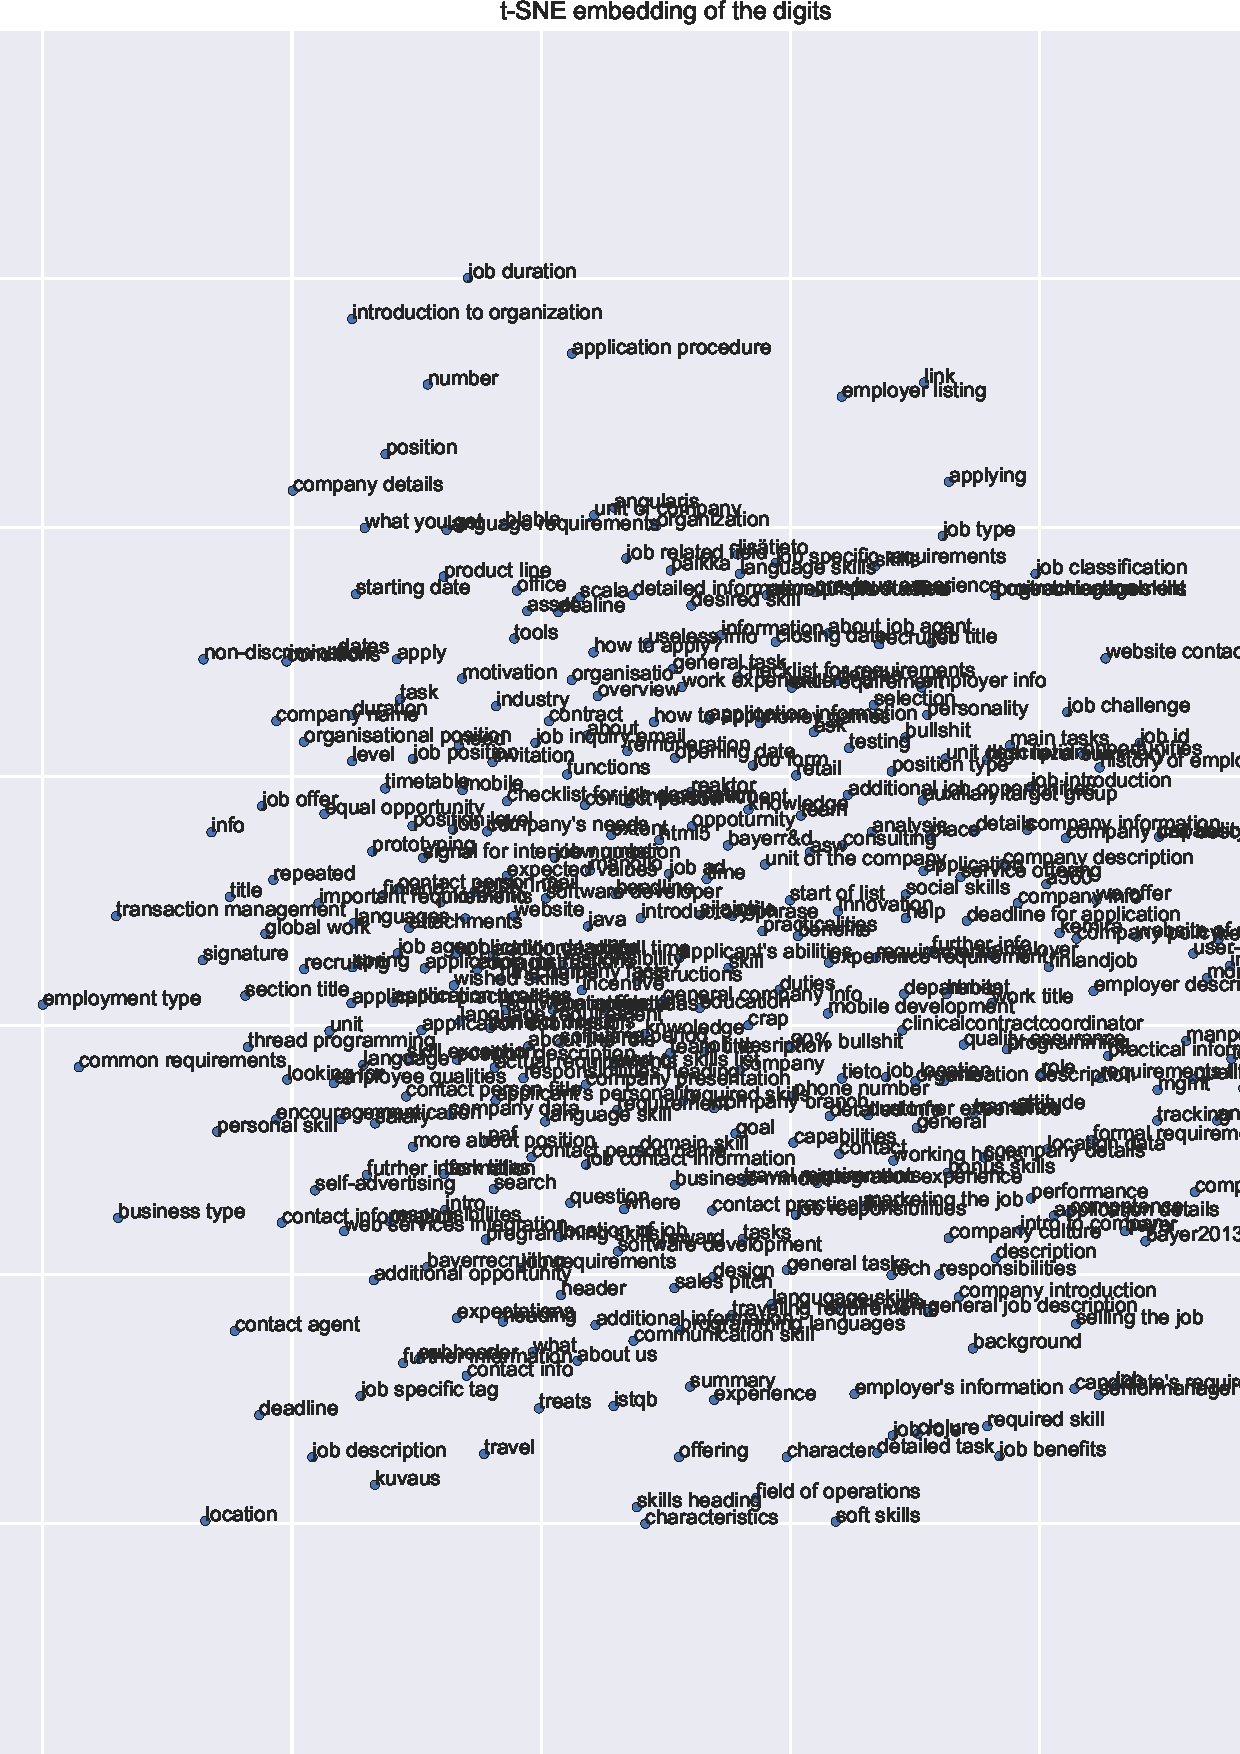
\includegraphics[width=\textwidth]{img/paragraph-data-tSNE.pdf}
    \caption{t-SNE Embedding}
\label{fig:paragraph-data-tSNE}
\end{figure}

\begin{figure}[h]
    \centering
    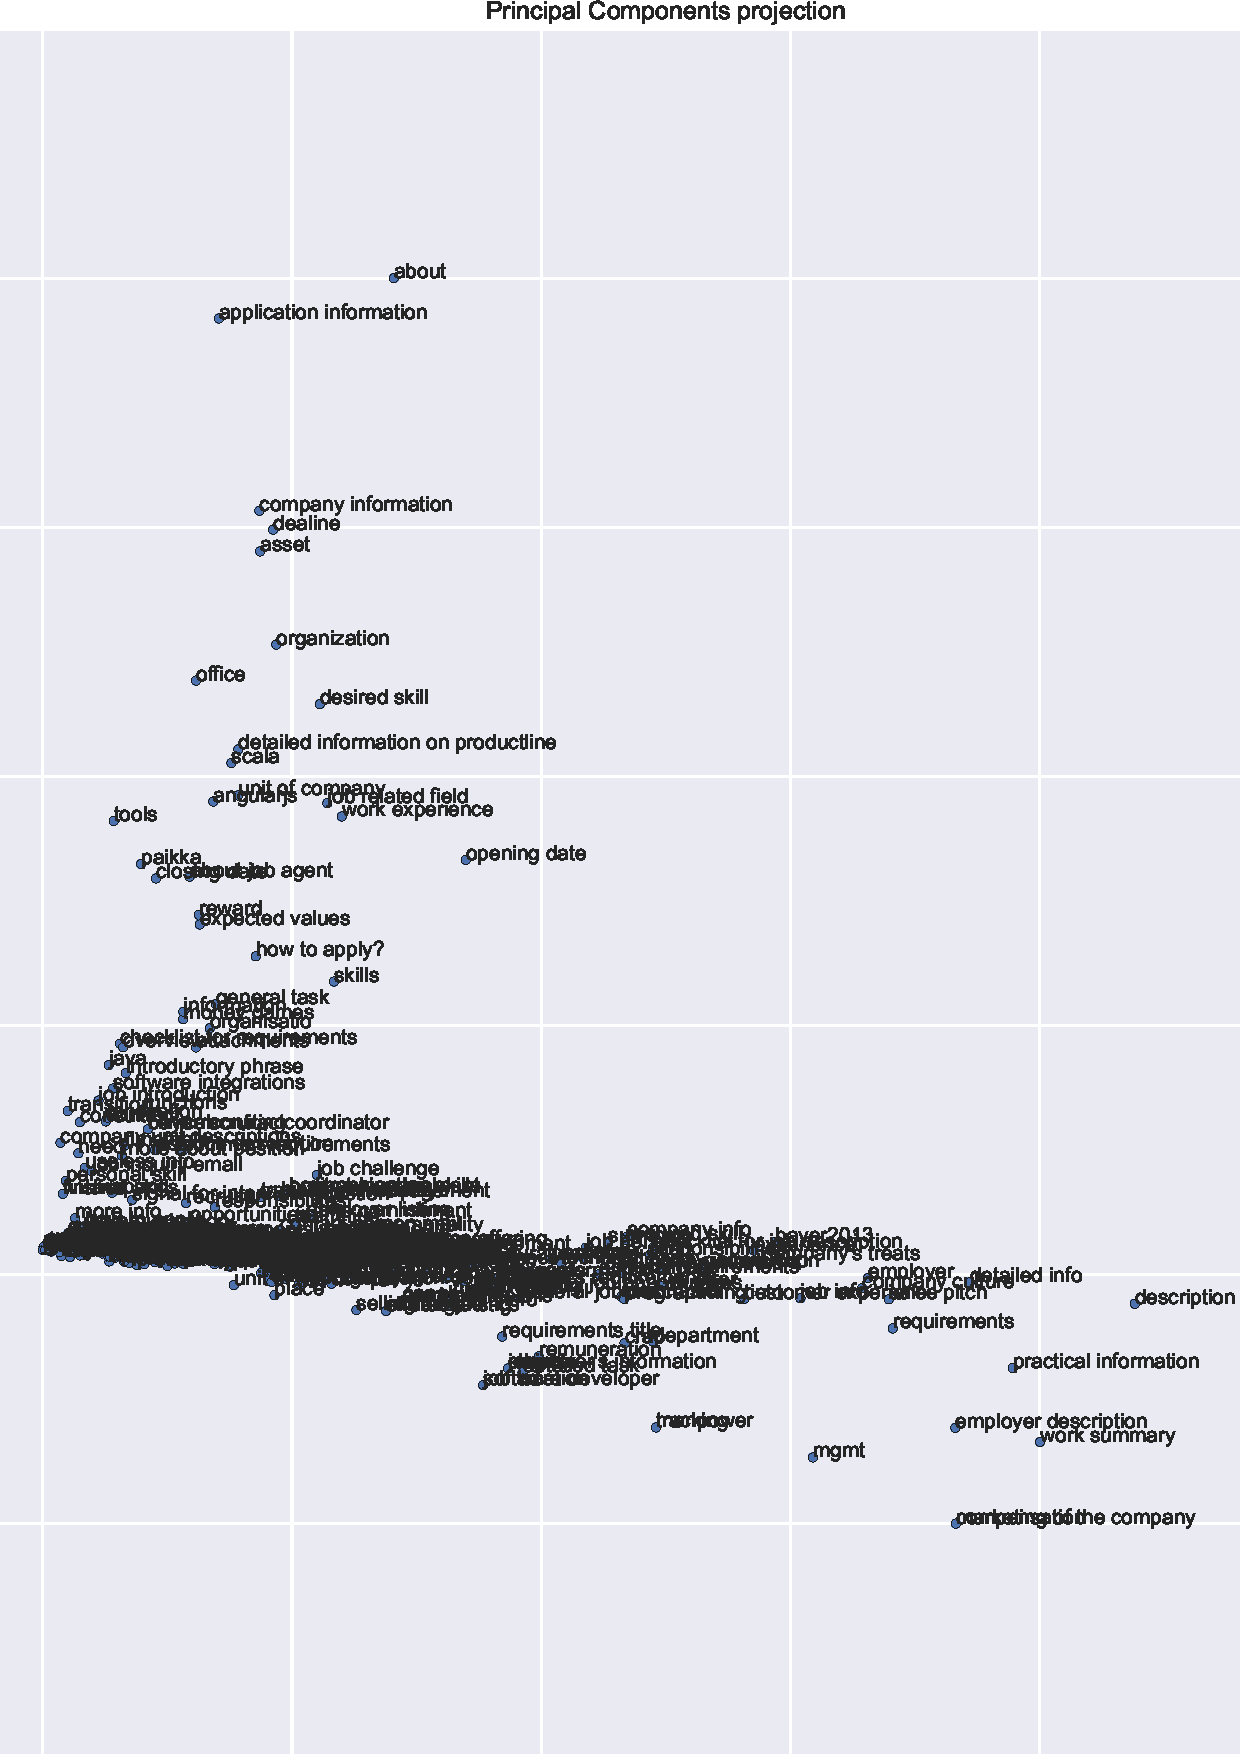
\includegraphics[width=\textwidth]{img/paragraph-data-principal-components-projection.pdf}
    \caption{Principal Components Projection}
\label{fig:paragraph-data-principal-components-projection}
\end{figure}

\todo{Comparison one-vs-rest and one-vs-one against linear machine}
\todo{Visualizations and embeddings of data in 2D (and decision boundaries?)}
\todo{show T-SNE embeddings of doc2vec vectors}


\subsection{Dataset 2}

\begin{figure}[h]
 % From http://localhost:8888/notebooks/thesis/experiments/vector-space-models/Vector%20Space%20Models.ipynb#Setup
    \centering
    \begin{subfigure}[b]{0.46\textwidth}
        \includegraphics[width=\textwidth]{img/sentence-data-judgement-confidence.pdf}
        \caption{Confidence}
\label{fig:sentence-data-judgement-confidence}
    \end{subfigure}
~%add desired spacing between images, e. g. ~, \quad, \qquad, \hfill etc.
    %(or a blank line to force the subfigure onto a new line)
    \begin{subfigure}[b]{0.43\textwidth}
        \includegraphics[width=\textwidth]{img/sentence-data-judgement-confidence-cumulative.pdf}
        \caption{Cumulative Confidence}
\label{fig:sentence-data-judgement-confidence-cumulative}
    \end{subfigure}
    \caption{Amount of label judgements versus label confidence of the sentence label data collected via crowdflower}
\label{fig:sentence-data-judgements}
\end{figure}



\begin{figure}[h]
  % From http://localhost:8888/notebooks/thesis/experiments/vector-space-models/Vector%20Space%20Models.ipynb#Setup
    \centering
    \includegraphics[width=\textwidth]{img/sentence-data-label-dist.pdf}
    \caption{Distribution of labels in sentence data}
\label{fig:sentence-data-label-dist}
\end{figure}

\section{Problem Definition: Text Classification}
\label{sec:Problem Definition: Text Classification}

\include{./tex/problem_def}
% !TEX root = ../thesis.tex
% !TEX spellcheck = en-US

\clearpage

\section{Methods}
\label{sec:Methods}

This chapter will provide the necessary background on text classification, assuming the reader is familiar with the basic concepts of Machine Learning and related fields. First the research problem will be defined. Then

Concepts:
\begin{itemize}
  \item likelihood
  \item function estimation
  \item linear algebra
  \item basic probabilistic and baysian terms (posteriors and priors)
  \item decision theory
  \item information theory
\end{itemize}

\subsection{Overview}
\label{sub:Overview}

\paragraph{Feature Space Construction}
\label{par:Space Construction Pipeline}

- vector space models with ngrams

\paragraph{Representation Learning}
\label{par:Representation Learning for Feature Spaces}

- learning embeddings via distributed representations

\paragraph{Deep Sequential Learning}
\label{par:Deep Sequential Learning}

- learning embeddings on the fly
- sequential modeling


% - vector space models: same principle as feature space construction in other typical ML pipelines
% - sequential approach more direct?

% \subsection{Approaches to Text Classification *}

% \subsubsection{Text as a Sequential Signal}
% \label{par:Text as a Sequential Signal}

% Text can be seen as a sequential signal like any other. Depending on the task at hand the resolution of this signal can be chosen more or less fine-grained, ranging from single characters to words, sentences, paragraphs or whole documents. The more fine-grained we choose our model to operate, the more sequential correlation we usually find, as characters, words tend to follow linguistic rules that constrain in which order combinations they can be used, and even sentences and paragraphs are often semantically related. This observation motivates the use of language models for the text classification task as will be discussed in Section \todo{reference}.

\subsection{Vector Space Models}
\label{sub:Vector Space Models}

Text documents cannot be used directly as input to a classifier, and are thus usually mapped into a vector space so that each document can be represented by a vector $\mathbf{v} \in \mathbb{R}^d$. This procedure is also known as \emph{Document Indexing}~\cite{Sebastiani:2002aa}.


\textquote{Contiguity hypothesis. Documents in the same class form a contiguous region and regions of different classes do not overlap.}~\cite[Chapter 14, p.~289]{Manning:2008aa}

Vector space model~\cite[Chapter 6.3, p.~120]{Manning:2008aa}

\textquote{the document `Mary is quicker than John' is, in this view, identical to the document `John is quicker than Mary'}\cite[Chapter 6.2, p.~117]{Manning:2008aa}


\subsubsection{N-gram Models}
\label{subs:N-gram Models}

N-gram language models are based on co-occurrences of word or character sequences, so-called N-grams or $k$-shingles as they are referred to in the Data Mining literature~\cite[Chapter 3.2, p.~72]{Leskovec:2014aa}. Formally an N-gram is defined as a sequence of $n$ items, each of which consist of $n$ characters or words, effectively used to capture sub-sequences of text. Common choices are N-grams of size 1, 2 or 3 --- called \emph{unigrams}, \emph{bigrams} and \emph{trigrams} respectively --- and the definition can be extended to using a window size $[\textit{w}_{\text{min}}, \textit{w}_{\text{max}}]$, employing all combinations of N-grams in this interval.

N-grams are usually used to create a vector-space model by representing each document in a dataset as a \textit{bag-of-words} or \textit{bag-of-N-grams} vector so that each dimension of the vector represents statistics about the corresponding N-gram. Specifically, a common way to compute the word count vectors for a document is the following:

\begin{equation}
  \text{TF}_{ij} = \frac{f_{ij}}{\max_k f_{kj}}
\end{equation}

Where $f_{ij}$ is \textquote{the \emph{frequency} (number of occurences) of a term (word) $i$ in document $j$} and $\text{TF}_{if}$ is the \emph{term frequency}, i.e.   \textquote{$f_{ij}$ normalized by dividing it by the maximum number of occurrences of any term [\ldots] in the same document}~\cite[Chapter 1.3.1, p.~8]{Leskovec:2014aa}.

\todo{example with 2 vectors and showing what they encode?}

\paragraph{Variants}

As this approach has been studied for decades \todo{citation for first or review paper here?} there is quite an extensive amount of variants and thus hyper-parameters to tune. The most important ones will be explained in the following sections:

\subparagraph{Words vs. Characters} The first choice when building an N-gram language model is to use characters or words as the atomic unit. In practically every case there are less characters than words in a dataset, but to capture expressive substrings usually larger N-gram window sizes or ranges have to be chosen, which leads to a combinatorial explosion. In case of word-based models on the other hand the maximal size of the feature space is the size of the vocabulary $\mathcal{V}$ in the case of unigrams or $V^k$ in case of $k$-grams.

\subparagraph{Stop words}
\label{subp:Stop words}
For creating N-gram models, so-called stop word lists are often used which are lists of frequent words that will be excluded as they do not carry much meaning~\cite[Chapter 1.3.1, p.~7]{Leskovec:2014aa}. The stop-word list used in these experiments is the standard list used for the Scikit-learn framework~\cite{Pedregosa:2011aa} which is a list gathered by the University of Glasgow Information Retrieval group\footnote{\url{http://www.gla.ac.uk/schools/computing/research/researchoverview/informationretrieval/}. The full stop word list can be found at \url{http://ir.dcs.gla.ac.uk/resources/linguistic_utils/stop_words} and in the appendix in Section~\ref{sec:appendix-stopwords}.}.

\subparagraph{N-gram range} The N-gram range, also known as window size or shingle size, refers to combinations of the atomic units of the model (words or characters) and defines an upper and lower limit for these combinations. For example a range of $[1,1]$ specifies a unigram model, $[2,2]$ a bigram model and $[1,2]$ a combination of both including all unigrams and all bigrams.
A larger range allows the model to capture an increasing amount of word order and thus context, but again leads to a combinatorial explosion in terms of feature space.

\subparagraph{Vector size} The vector size imposes an upper limit to the vector size and therefor the number of N-grams that can be encoded in the feature space. Commonly this simply uses the words with the highest frequency to reduce the vector size from the full length --- the size of the vocabulary --- to the desired size.

\subparagraph{TF.IDF weighting}
\label{subp:TF.IDF weighting}
A common extension to using word-counts is to weight the term frequencies by the so-called inverse document frequency, i.e.\ the inverse of the frequency of an term or N-gram in all documents. This method is commonly referred to as \emph{TF.IDF} and specifically the inverse document frequency is defined as $\text{IDF}_i = \log_2 (N/n_i)$, where logarithmic smoothing is applied. The TF.IDF value for a term or N-gram is then computed as $\text{TF}_{ij} \cdot \text{IDF}_i$.

\subparagraph{Sublinear TF scaling}
\label{subp:Sublinear TF scaling}
 As~\cite[Chapter 6.4.1, p.~126]{Manning:2008aa} suggests \textquote{[it] seems unlikely that twenty occurrences of a term in a document truly carry twenty times the significance of a single occurrence}. Hence a common variant is \emph{sublinear scaling} where we down-weigh the increase in term importance by applying a logarithmic function to it, resulting in the sub-linear term frequency $\text{subTF}_{ij}$:

\begin{displaymath}
  \text{subTF}_{ij} = \left \{ \begin{array}{l l} 1+\log \text{TF}_{ij} & \text{TF}_{ij} > 0 \\
  0 & \text{otherwise}
\end{array} \right \}
\end{displaymath}

\subparagraph{Normalization} Often the term vectors are globally normalized using the $L_1$ or $L_2$ norm to remove the effect of statistical differences between the terms.

There are, of course, various other variants and modifications to the N-gram model, but within the scope of this thesis only the most notable ones were introduced and will be used for experiments later. For further material on this subject refer for example to~\cite{Manning:2008aa}.

\todo{mention smoothing techniques~\cite{Chen:1996aa}}

\paragraph{Shortcomings}
\label{subs:shortcomings-ngrams}

Today N-gram models are still in wide use and considered as state of the art \textquote{not because there are no better techniques, but because those better techniques are computationally much more complex, and provide just marginal improvements}~\cite[p.~17]{Mikolov:2012aa}. As~\cite{Mikolov:2012aa} points out further \textquote{[the] most important weakness is that the number of possible n-grams increases exponentially with the length of the context, preventing these models to effectively capture longer context patterns. This is especially painful if large amounts of training data are available, as much of the patterns from the training data cannot be effectively represented by n-grams and cannot be thus discovered during training. The idea of using neural network based LMs [Language Models] is based on this observation, and tries to overcome the exponential increase of parameters by sharing parameters among similar events, no longer requiring exact match of the history H.}~\cite[p.~17]{Mikolov:2012aa}

\subsubsection{Learned Distributed Continuous Representations}
\label{subs:Learned Distributed Continuous Representations}

To overcome the shortcomings of popular language models such as the ones of the N-gram model mentioned above, lots of recent work went into the study of so-called distributed language models. One branch of research that gained significant attention is the work on Neural Network based Language models (NNLMs), popularized largely through the work of T. Mikolov and his software realization of such a model dubbed \emph{word2vec} with interest coming not only from the academic community. His work builds on ideas introduced in~\cite{Bengio:2000aa} where a neural network based model was proposed for modeling high-dimensional discrete data, which was then applied to the domain of language modeling in~\cite{bengio2003neural}. Following the description in this paper, the approach is as follows:

\begin{enumerate}
  \item Associate with each word in the vocabulary a distributed \emph{word feature vector} (a real-valued vector in $\mathbb{R}^m$),
  \item Express the joint \emph{probability function} of word sequences in terms of the feature vectors of these words in the sequence, and
  \item Learn simultaneously the \emph{word feature vectors} and the parameters of that \emph{probability function}.
\end{enumerate}

To achieve this, a feedforward neural network model is trained to learn these \emph{word feature vectors} or \emph{word embeddings}. As input a sequence of $n$ words is given, each encoded using one-hot encoding or one-of-$V$ encoding where the corresponding indicator vectors for each word have the size of the vocabulary $V$. The input word vectors are then projected linearly into a projection layer of significantly lower dimensionality $D$, using a global projection matrix for across all words, and concatenated, forming the input of size $D \times N$ to a hidden layer of size $H$. The hidden layer then feeds non-linearly into the output layer that is again of size $V$, modeling the probability distribution for a word given its context $P(w_t \mid w_{t - n}, \ldots, w_{t - 2}, w_{t - 1})$.

\paragraph{Simplified Continuous Models}

\cite{Mikolov:2013ad} then introduced two simplified models, removing the hidden layer and only using a projection layer, with shared weights for all words. The Continuous Bag-of-Words Model (CBOW) model is trained to predict the current word $w_t$ given the $k$ words around it. Its name is due to the fact that the word order does not influence the projection as the word vectors are summed or averaged. The Continuous Skip-gram Model works the other way around, predicting the most likely $k$ words around a given word $w_t$. Figure~\ref{fig:cbow-skip-gram} illustrates both models.

\begin{figure}[h]
    \centering
    \begin{subfigure}[b]{0.49\textwidth}
        \includegraphics[width=\textwidth]{img/cbow_vert2.pdf}
        \caption{Continuous Bag-of-Words Model}
\label{fig:cbow}
    \end{subfigure}
    %add desired spacing between images, e. g. ~, \quad, \qquad, \hfill etc.
      %(or a blank line to force the subfigure onto a new line)
    \begin{subfigure}[b]{0.49\textwidth}
        \includegraphics[width=\textwidth]{img/skip-gram_vert2.pdf}
        \caption{Continuous Skip-gram Model}
\label{fig:skip-gram}
    \end{subfigure}
    \caption{Architectures for learning continouus distributed word vectors, adapted from~\cite{Mikolov:2013ad}}
\label{fig:cbow-skip-gram}
\end{figure}

\begin{wrapfigure}{l}{0.6\textwidth}
  \begin{center}
    \includegraphics[width=0.58\textwidth]{img/word2vec_cities.pdf}
  \end{center}
  \caption{Two-dimensional PCA projection of the 1000-dimensional Skip-gram vectors of countries and their capital cities. The figure illustrates ability of the model to automatically organize concepts and learn implicitly the relationships between them, as during the training we did not provide any supervised information about what a capital city means. (Adapted from~\cite{Mikolov:2013ac})}
\label{fig:word2vec-cities}
\end{wrapfigure}

These models have been shown to outperform state of the art N-gram models on various tasks (see e.g.~\cite{bengio2003neural} or~\cite{Mikolov:2012aa}). An interesting outcome of this research is the fact that these \emph{word vectors} capture many interesting and often subtle semantic regularities and that these can be exploited explicitly in an algebraic manner. When trained on an extensive dataset, one can perform calculations as $v(Paris) - v(France) + v(Germany)$ and the closest vector to the result turns out to be $v(Berlin)$ where $v(\cdot)$ denotes the \emph{word vector} of a word. Figure~\ref{fig:word2vec-cities} shows a PCA projection of Skip-gram trained vectors of countries and their capital cities.

A notable alternative to these models was developed by~\cite{Pennington:2014aa}. In their model called \emph{GloVe}, which stands for global vectors, they construct a vector space model with similar properties as the models introduced above, which instead relies global word-word co-occurrence counts. This method thus operates directly in the co-occurrence statistics of the corpus compared to the Neural Network based methods that \textquote{fail[\ldots] to take advantage of the vast amount of repetition in the data}~\cite{Pennington:2014aa}.

There have been various extensions and variants to the Neural Network based language models especially, including architectures based on Recurrent Neural Networks (see~\cite{Mikolov:2012aa}). Some of the most important variations will are discussed in the following section as they were evaluated in the experiments:

\subparagraph{Hierarchical Softmax}
The architectures proposed in~\cite{Bengio:2000aa},~\cite{bengio2003neural} and follow-up work use a \emph{softmax} activation function at the output layer in order to obtain valid probabilities for each word to be predicted:

\begin{equation}
  \operatorname{softmax}(\mathbf{x}_j) = \frac{\exp(\mathbf{x}_j)}{\sum_k \exp(\mathbf{x}_k)}
\end{equation}

\emph{Hierarchical Softmax} uses a binary tree to encode the output which leads to an efficient approximation of the full softmax and speeds up training and inference. Details can be found in~\cite{Mikolov:2013ab}.

\subparagraph{Negative Sampling}
Another technique applied by~\cite{Mikolov:2013ab} \emph{Negative Sampling} which is a simplified version of Noise Contrastive Estimation (NCE) introduced by~\cite{Gutmann:2012aa}. Based on the insight that a good model should be able separate noise from signal, this method mixes samples from a noise distribution into the signal to be learned, in this case random words that are not in the context window, which is shown to approximately maximize the log probability of the softmax. Free parameters of this technique are the number of negative samples $k$ per data sample and the noise distribution $P_n(w)$

\subparagraph{Sub-sampling of Frequent Words}
As there the difference between frequent and infrequent words in large corpora can be huge and the frequent words often don't carry as much meaning, in~\cite{Mikolov:2013ab} a simple sub-sampling technique is used to counter this imbalance by discarding words with a probability computed as follows:

\begin{equation}
  P(w_i) = 1 - \sqrt{\frac{t}{f(w_f)}}
\end{equation}

with $f(w_i)$ denoting the frequency of word $w_i$ and $t$ denoting a threshold.~\cite{Mikolov:2013ab} state that this method, while chosen heuristically, \textquote{accelerates learning and even significantly improves the accuracy of the learned vectors of the rare words}.

\paragraph{Distributed representations for documents}
\label{par:Distributed representations for documents}

The models explained above are defined on words as the atomic unit. Therefore several ways have been proposed to extend these to sequences of words in order to obtain a vector space of sentences or documents. A few of these will be briefly outlined here:

\subparagraph{Bag-of-Means}
\label{subp:Bag-of-Means}
The term \emph{Bag-of-Means} refers to simply averaging over the word embedding vectors of all words in a document. However this approach \textquote{loses the word order in the same way as the standard bag-of-words models do.}~\cite{Le:2014aa}. This intuitive property was confirmed by~\cite{Zhang:2015aa} where the method consistently performed poorest in comparison to other approaches on a variety on tasks.

\subparagraph{Parse Trees}~\cite{Le:2014aa} also mention a more sophisticated approach by \textquote{combining the word vectors in an order given by a parse tree of a sentence.} as done in~\cite{Socher:2011aa}, with the disadvantage that this method \textquote{has been shown to work for only sentences because it relies on parsing}~\cite{Le:2014aa}.

\subparagraph{Paragraph Vectors *}
In~\cite{Le:2014aa} a different approach is shown that builds on the same idea as the original word2vec model:

\subsection{Classification Methods using Vector Space Models}
\label{sub:Classification Methods using Vector Space Models}

Many classical machine learning algorithms work on data in a fixed-dimensional vector format and can thus be applied to a vector space model as described in the previous section. Here a set of well-known algorithms will be briefly introduced, each representing a family of approaches with different model assumptions. It should be pointed out that there exist a plethora of other models and algorithms that can be used, the ones chosen here though are widely considered standard methods and have proven successfully in the past for a wide range of problems.

% \paragraph{Classification Schemes}
% \label{par:Classification Schemes}
% There are three common schemes for classification: In \emph{binary classification} there is only a single class and for each document we decide whether or not it belongs to this class. A classic example is email spam detection where we predict if a given email is spam or not. \emph{Multi-class classification} assumes the existence of more than one class and can be sub-categorized into \emph{single-label classification} where the labels are mutually exclusive and and \emph{multi-label classificaion} where they are not and thus multiple labels can be assigned to a single document at the same time. These settings also need be evaluated differently which will be discussed in Section~\ref{sub:Evaluation}.




% A simple approach to multi-class classification is to pose the learning problem as a combination of binary classification problems as described in~\cite[Chapter 4.1.2, p.~182]{Bishop:2006aa}. This can be done by using $K$ separate classifiers, each of which predicts one of the classes against all $K-1$ other classes, which is known as the \textit{one-versus-the-rest} classification scheme. An alternative approach is to train $K (K - 1) / 2$ binary classifiers for each possible pair of classes, referred to as \textit{one-versus-one} classification.
%
% These extensions though have major drawbacks as pointed out by~\cite[Chapter 5.2.2]{Duda:1973aa}. As illustrated by~\ref{fig:Bishop2006aa-p182-ch4-fig4-1} both of the classification schemes lead to ambiguous regions in the hypothesis space as their classification is undefined.
%
% \begin{figure}[h]
%     \centering
%     \begin{subfigure}[b]{0.4\textwidth}
%         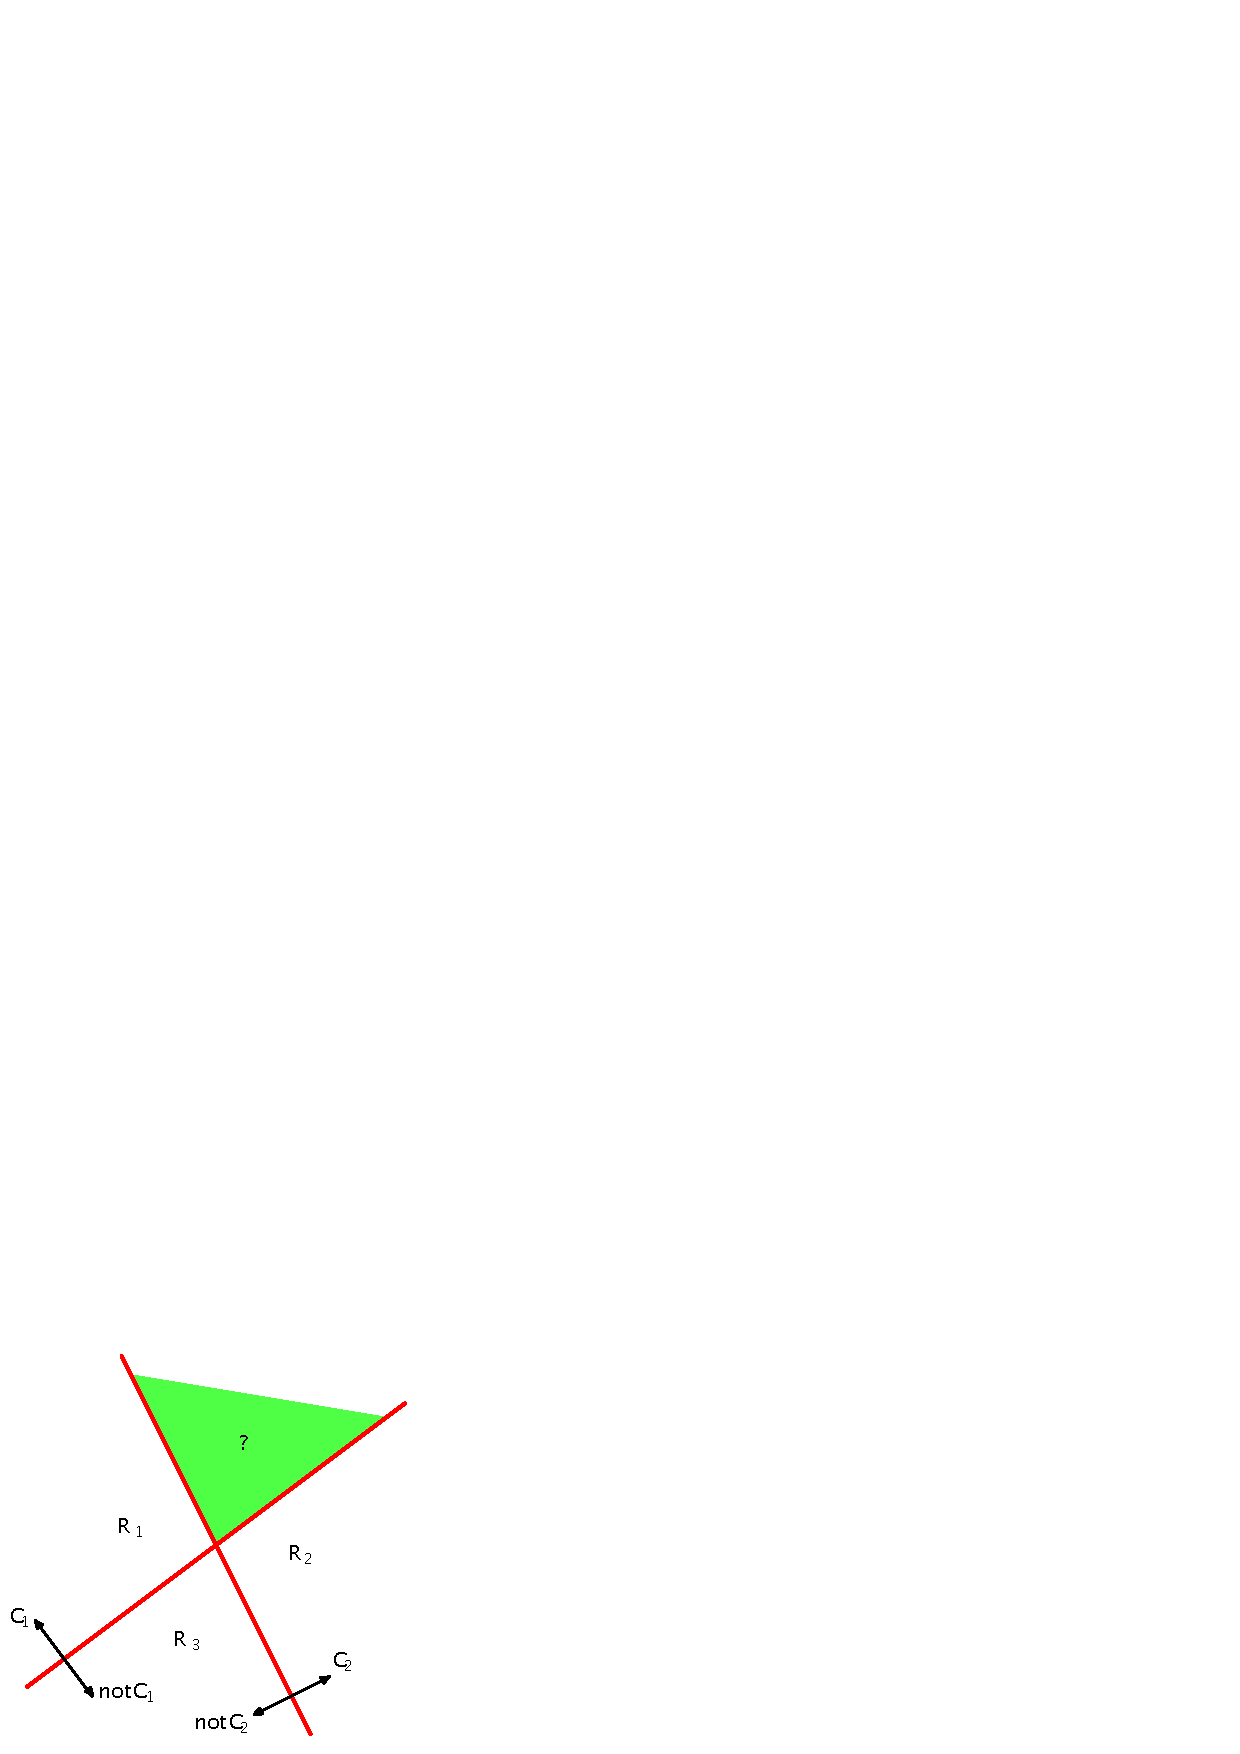
\includegraphics[width=\textwidth]{img/Bishop2006aa-p182-ch4-fig4-1-a.pdf}
%         \caption{One-Vs-Rest classification scheme}
%         \label{fig:Bishop2006aa-p182-ch4-fig4-1-a}
%     \end{subfigure}
%     ~ %add desired spacing between images, e. g. ~, \quad, \qquad, \hfill etc.
%       %(or a blank line to force the subfigure onto a new line)
%     \begin{subfigure}[b]{0.4\textwidth}
%         \includegraphics[width=\textwidth]{img/Bishop2006aa-p182-ch4-fig4-1-b.pdf}
%         \caption{One-Vs-One classification scheme}
%         \label{fig:Bishop2006aa-p182-ch4-fig4-1-b}
%     \end{subfigure}
%     \caption{: Ambiguous regions in the hypothesis space (\cite{Bishop:2006aa} Chapter 4, Figure 4.1) }
%     \label{fig:Bishop2006aa-p182-ch4-fig4-1}
% \end{figure}

\subsubsection{Generalized Linear Models}
\label{subs:Generalized Linear Modelsl}

Generalized Linear Models are an extension of linear discriminant functions. Whereas discriminant functions and ordinary linear regression models produce linear decision boundaries in the input space (\emph{linear-response model}), Generalized Linear Models apply a non-linear \emph{link function} or \emph{basis function} to the input, making it possible for the model to achieve non-linear decision boundaries in the original input space while corresponding to a linear decision boundary in the feature space.

The most prominent algorithm in this class is \emph{Logistic Regression} which uses the \emph{logistic sigmoid} function as a basis function:

\begin{equation}
  \sigma (a) = \frac{1}{1 + \exp(-a)}
\end{equation}

This yields posterior class probabilities of:

\begin{equation}
  p(\mathcal{C}_n \mid \phi) = y(\phi) = \sigma(w^T  \phi)
\end{equation}

where $w$ is the learned \emph{weight vector} with the free parameters of the model, $\phi$ is the \emph{feature vector} of inputs transformed through the basis function $\sigma$ and $y$ is the model function that we use to infer class predictions from our data.

Using a the maximum likelihood method we can now find a set of parameters for our model function $y$ that gives us the predictions with the lowest error. For a dataset $\{ \phi_n, t_n \}$, where $t_m \in {0, 1}$ and $\phi_n = \phi(x_n)$, with $n = 1, . . ., N$ denoting the amount of data points:

\begin{equation}
  p(\mathbf{t} | w) = \prod_{n=1}^N y_n^{t_n} \{ 1 - y_n \}^{1-t_n}
\end{equation}

where $\mathbf{t} = (t_1, \ldots, t_N)^T$ and $y_n = p(\mathcal{C}_n \mid \phi)$. We can now define an error function by taking the negative logatirhm of the likelihood, which is called the \emph{cross-entropy} error function:

\begin{equation}
  E(\mathbf(w)) = - \ln p(\mathbf{t} | w) = - \sum_{n=1}^N \{ t_n \ln y_n + (1 - t_n) \ln (1-y_n) \}
\end{equation}

where $y_n = \sigma(a_n)$ and $a_n = \mathbf{w}^T \phi_n$. When taking the gradient we with resepect to $\mathbf{w}$ we obtain:

\begin{equation}
  \nabla E(\mathbf{w}) = \sum_{n=1}^N (y_n - t_n) \phi_n
\end{equation}

From here we can apply an optimization procedure such as gradient descent to arrive at a weight vector $\mathbf{w}$ that minimizes the error function above. A deeper treatment of the Logistic Regression and Generalized Linear Models can be found in many introductory textbooks such as~\cite[Chapter 4.3.2, p.~205]{Bishop:2006aa}.

\todo{extension to multinomial?}

\subsubsection{Bayesian Classifiers}
\label{subs:Bayesian Classifiers}

Bayesian Classifiers are a family of probabilistic models derived from Bayes' Theorem, which itself is a simple application of the rule conditional probability:

\begin{equation}
  p(A \mid B) = \frac{P(B \mid A) P(A)}{P(B)}
\end{equation}

Where $P(A)$ is the probability of A and $P(A \mid B)$ conditional probability of A given B. In the Bayesian interpretation probabilities represent a degree of belief that changes under the observation of evidence. The following form is usually referred to as Bayes' rule and expresses this interpretation:

\begin{equation}
  \underbrace{p(A \mid B)}_{posterior}  \propto \underbrace{P(B \mid A)}_{likelihood} \underbrace{P(A)}_{prior}
\end{equation}

where $P(B)$ is marginalized out as a normalization constant of the probabilities. This simple rule forms the basis of a whole subfield of Bayesian Inference (see e.g.\ the textbook~\cite{Barber:2012aa} for a good coverage of the topic).

The most known Bayesian classification algorithm is the \emph{Naive Bayes} classifier, a simple class-conditional generative model which builds on the assumption that all data points are conditionally independent given the classes $\mathcal{C}_n$. For each class $c_j$ we can predict it's probability given an input vector $\mathbf{x}$ as:

\begin{equation}
  p(\mathbf{x}) = p(c_j) \prod_{i=D}^D p(x_i \mid c_j)
\end{equation}

We can then use Bayes' rule to form a classifier for each class:

\begin{equation}
  p(c_j \mid \mathbf{x}) = \frac{p(\mathbf{x} \mid c_j ) p(c_j)}{ p (\mathbf{x})} = \frac{p(\mathbf{x} \mid c_j ) p(c_j)}{ \sum_c p(\mathbf{x \mid c} p(c)) }
\end{equation}

We can then choose the class with the highest class probability as our prediction. Again there are numerous variants and related models to Naive Bayes and it can be regarded as a simple \emph{graphical model}, a family of techniques which are covered e.g.\ in~\cite{Barber:2012aa} or~\cite{Bishop:2006aa}.

\todo{more on ML estimation?}

\subsubsection{Tree Based Methods}
\label{subs:Tree Based Methods}

\begin{wrapfigure}{r}{0.5\textwidth}
  \centering
  \includegraphics[width=0.48\textwidth]{img/decision-tree.pdf}
  \caption{A simple Decision Tree to determine whether a building is located in New York (NY) or San Francisco (SF).}
\label{fig:decision-tree}
\end{wrapfigure}

A simple but widely used classification as well as regression method are \emph{Decision Trees} which work by recursively partitioning the input space into dichotomous subregions, producing a binary decision tree. At inference time the resulting tree can then be used to produce an output by navigating through a path from its root to a leaf, answering a binary questions at each node to determine which child node to query next. Figure~\ref{fig:decision-tree} shows the visualization of an exemplified such a tree\footnote{Adapted from R2D3's great visual introduction to Machine Learning at \url{http://www.r2d3.us/visual-intro-to-machine-learning-part-1/}}.
Every node represents a threshold in the input space that  the input data is compared against, corresponding to a decision such as ``Is the elevation of this building's elevation higher than or equal to 91.9 feet?''. If the answer is ``Yes'' the left child node is queried next, otherwise the right. This procedure is repeated until a leaf with a final answer is reached.

The technique was first introduced by~\cite{Breiman:1984ab} under the term \emph{Classification And Regression Tree (CART)} but exists in many variants. Learning such a model involves specifying the structure of the tree, including which input variable to query at each node in the graph and what each of the nodes' threshold values are. Since commonly it is computationally infeasible to generate and evaluate all possible decision trees for a given problem, a greedy procedure is usually chosen. We start with determining a first split in the data that represents the root node and grow the tree one node at a time, each node in the tree being determined by choosing splits that minimize an error measure.

Let $p_{\tau k}$ be the proportion of data points in region $R_{\tau}$ that are assigned to class $k$. Then we define the error as the negative cross-entropy:

\begin{equation}
  Q_{\tau}(T) = \sum_{k=1}^K p_{\tau k} \ln p_{\tau k}
\end{equation}

A common alternative for the classification error is the \emph{Gini index}:

\begin{equation}
  Q_{\tau}(T) = \sum_{k=1}^K p_{\tau k} (1 - p_{\tau k})
\end{equation}

Both measures vanish for $p_{\tau k} = 0$ and $p_{\tau k} = 1$ and are maximal at $p_{\tau k} = 0.5$, thus rewarding regions with a high proportion of data points assigned to one class. As~\cite[Chapter 14.4, p.~664]{Bishop:2006aa} notices \textquote{cross entropy and the Gini index are better measures than misclassification rate for growing the trees because they are more sensitive to the node probabilities. Also, unlike misclassification rate, they are differentiable and hence better suited to gradient based optimization methods}.

Decision trees are often chosen because they introduces next to no inductive model bias, but one has to be aware that this leads to high variance due to the Bias-Variance Dilemma. The algorithm is this prone to overfitting which is often countered by pruning, using a criterion that balances error with model complexity, such as:

\begin{equation}
  C(T) = \sum_{\tau=1}^{|T|} Q_{\tau}(T) + \lambda |T|
\end{equation}

Where $\lambda$ is a regularization parameter. Pruning of the tree happens after training a full tree as evidence shows that sometimes several splits occur that do not significantly reduce the error, followed by one that does~\cite[Chapter 14.4, p.~664]{Bishop:2006aa}.

\subsubsection{Ensemble Methods}
\label{subs:Ensemble Methods}

Another approach to machine learning algorithms are so-called \glspl{Ensemble Method}. These methods use different strategies to combine a set of classifiers, often employing techniques of \glspl{Randomized Algorithm}. There is a variety of such algorithms including \gls{Bagging}, \gls{Boosting} and \gls{Voting} methods which are covered in most of the popular introductory books to machine learning, e.g.~\cite{Bishop:2006aa}.

The Random Forests learning algorithm is a popular \gls{Ensemble Method} introduced by~\cite{Breiman:aa}. It is based on the concept of Decision Trees explained above, but instead of a single decision tree a set of trees, i.e.\ a forest, is grown on sets of bootstrapped samples from the input space. Specifically the algorithm grows $b = 1 \ldots B$ random trees by repeating the following steps for $b$ iterations:

\begin{enumerate}
  \item A \emph{bootstrapped sample} $S_i$ of data points is generated by drawing samples uniformly at random with replacement from the original data $D$. The sample is of smaller size than the dataset and is thus based on a subset of the input data. Notice that data can be sampled multiple times.
  \item A decision tree $T_i$ is trained on the bootstrapped data sample and is usually pruned at a certain limit of nodes.
\end{enumerate}

Then the resulting forest of trees ${T_1, \ldots, T_b}$ is used as an ensemble of classifiers using a majority vote over the predictions:

\begin{equation}
  C(X) = \frac{1}{B} \argmax_i \sum_{b = 1}^B \mathcal{I}(y_{T_b} = i)
\end{equation}

Where $\mathcal{I}(\cdot)$ is the indicator function. Other voting schemes have been proposed as well \todo{such as \ldots}.

\subsubsection{Instance-based Methods}
\label{subs:Instance-based Methods}

Another common class of learning algorithms are \emph{instance-based learning methods}, also known as \emph{example-based methods} or \emph{memory-based learning methods}. These methods directly use the given training examples and comparing new unseen examples with the training data at inference time, thus constructing the hypothesis directly from the data.

One of the most prominent instance-based classification methods is the \gls{knn} algorithm which simply makes a class prediction based on the majority class amongst its $k$ nearest neighbors in the input space.

The choice for the parameter $k$ depends on the type of problem and is often determined empirically via hyper-parameter optimization\todo{glossary?} or based on heuristics. The \gls{knn} algorithm is highly prone to the curse of dimensionality as when a metric such as the Euclidean Distance is used as a metric for the \gls{knn} algorithm to determine the nearest neighbors to the query vector there is little difference in the distance between samples in very high-dimensional spaces. Thus often \gls{Feature Extraction} or \gls{Dimensionality Reduction} techniques are employed before applying the \gls{knn} algorithm.

\subsubsection{Kernel Methods}
\label{subs:Kernel Methods}

\todo{rewrite a bit}

Kernel Methods can be seen as a set of instance-based methods (see Section~\ref{subs:Instance-based Methods}, as they construct the hypothesis using based on the training data. To achieve predictions on unseen data a similarity function $k$ between the training examples and the unseen data points is used. This function is called the \emph{kernel function} or simply \emph{kernel}, giving rise to the name of this class of these methods. The kernel function is chosen to be expressible as the inner product in another vector space $\mathcal{V}$. With a function adhering to this property a feature map $\varphi \colon {\mathcal {X}}\to {\mathcal {V}}$ can be constructed, satisfying:

\begin{equation}
  k(\mathbf {x} ,\mathbf {x'} )=\langle \varphi (\mathbf {x} ),\varphi (\mathbf {x'} )\rangle _{\mathcal {V}}.
\end{equation}

This avoids the explicit mapping that is needed to get linear learning algorithms to learn a nonlinear function or decision boundary.

The best known member of is the \gls{svm}.

\subsubsection{Neural Networks}
\label{subs:Neural Networks}

\gls{ANN} are a


\subsection{Sequential Text Classification}
\label{sub:Sequential Modeling Approach}

\cite{Gers:1999aa} --- Learning to forget: continual prediction with LSTM.

\subsection{Evaluation Metrics for Text Classification}
\label{sub:Evaluation Metrics for Text Classification}

In this section the basics of evaluating classification models for the given problem will be laid out. First the different evaluation schemes and their advantages or disadvantages are explained in the dichotomous case where only one class is to be predicted in terms of being active or not. Then these are generalized to the multi-label case where $K$ mutually exclusive classes are given. The last section extends this concept again towards so-called multi-label multi-output classification where several output labels can be predicted at the same time.

\subsubsection*{Binary Classification}
\label{subs:Binary Classification}

In the binary case of classification we are given a single class $k$ and a set of labelled data points $\mathcal{D} = \{ (x_1, y_1), (x_2, y_2), \ldots, (x_n, y_n) \}$ where targets $y_i \in \{0, 1\}$ encode whether a data point $x_i$ belongs the class $c$ or not. The task is then to achieve correct classification of new data points without knowing the true label via a model function or predictor $f(\cdot)$.

To evaluate such a predictor it is useful to present the results in form of a contingency table as shown in table Table~\ref{table:contingency-table-2}, because it gives valuable insights about the performance of the prediction. The table shows the proportion of data points that belong to the class (RP) or not (RN) and were predicted correctly (TP) or incorrectly (FN), as well as the number of data samples that do not belong to the class (RN) and were falsely predicted to be in the class (FP) or correctly predicted to not be in the class (TN), and the same proportions for the positively (PP) and negatively (PN) predicted cases with respect to the true assignments to the data. N refers to the total amount of data points.

\begin{table}[h]
  \begin{center}
    \begin{tabular}{r | c c }
      & Real Positives (RP) & Real Negatives (RN) \\
      \hline
      Predicted Positives (PP) & True Positives (TP) & False Positives (FP) \\
      Predicted Negatives (PN) & False Negatives (FN) & True Negatives (TN) \\
    \end{tabular}
  \caption{Contingency table for binary classification}
\label{table:contingency-table-2}
  \end{center}
\end{table}

\paragraph{Accuracy}
\label{par:Accuracy}

An intuitive choice towards classification is to simply ask which data points were correctly classified to belong to the class or not. In terms of the contingency table above the ratio of $(\text{TP} + \text{FP}) / (\text{N})$, commonly referred to as the ``accuracy'' of the classifier.

This choice can give a good intuition and it does capture the effectiveness on both true positives as well as true negatives, but it is strongly influenced by bias of the true and predicted class distribution (known as prevalence RP/N and label bias) as pointed out by~\cite{Powers:2011aa}. For example given a population of 900 positive and 100 negative examples, a predictor that simply always chooses a positive assignment can achieve accuracy of 90\% while it obviously is not a great predictor.

\textquote{There is a good reason why accuracy is not an appropriate measure for information retrieval problems. In almost all circumstances, the data is ex- tremely skewed: normally over 99.9\% of the documents are in the nonrele- vant category. A system tuned to maximize accuracy can appear to perform well by simply deeming all documents nonrelevant to all queries. Even if the system is quite good, trying to label some documents as relevant will almost always lead to a high rate of false positives. However, labeling all documents as nonrelevant is completely unsatisfying to an information retrieval system user. }\cite[Chapter 8.3, p.~155]{Manning:2008aa}

\paragraph{Precision, Recall and F1 Score}
\label{par:Precision, Recall and F1 Score}

In the field of Information Retrieval it is common practice to measure the effectiveness of a predictive system in terms of its precision and recall.
The precision of such system is \textquote{the proportion of retrieved material that is actually relevant} whereas the recall measures \textquote{proportion of relevant material actually retrieved in answer to a search request}~\cite{Rijsbergen:1979aa}. Formally these two measures are defined as:

\begin{equation}
    \text{Precision} = \frac{\text{TP}}{\text{TP} + \text{FP}}
\end{equation}
\begin{equation}
    \text{Recall} = \frac{\text{TP}}{\text{TP} + \text{FN}}
\end{equation}


As both, high precision and recall, are important for an robust information retrieval system they are typically combined into a single measure such as the F-measure, also referred to as F-score. The F-score is the weighted harmonic mean between precision and recall, derived from the measure of effectiveness proposed in~\cite{Rijsbergen:1979aa}. The most common form is the $F_1$ score  where precision and recall are assigned equal weight:
\begin{equation}
  \label{f1measure}
  F_1 = 2 \cdot \frac{\text{Precision} \cdot \text{Recall}}{\text{Precision} + \text{Recall}}
\end{equation}

The $F_1$ score has the advantage of its intuitive interpretability as both precision and recall are well understood measures and, analogous to recall, precision and accuracy, as it lives in the range $[0,1]$, giving a single number that can express the effectiveness of the system in terms of percentage.

The F1 score is widely used in the field of Machine Learning and Data Mining and thus it is an important measure to consider to compare results to outcomes of prior publications by others.
It is however important to point out that any version of the F-measure is a biased score as it \textquote{ignores TN which can vary freely without affecting the statistic}~\cite{Powers:2011aa}. This can affect the evaluation of a classifier when the class distribution is skewed (prevalence) or the classifier develops a bias towards certain classes (label bias), motivating the use of unbiased measures in these cases, such as the ones described next.

\paragraph{Informedness, Markedness and Matthews Correlation Coefficient}
\label{par:Informedness, Markedness and Matthews Correlation Coefficient}

\cite{Powers:2011aa} introduces unbiased analogue measures to Recall and Precision, called ``Informedness'' and ``Markedness'' respectively. As~\cite{Powers:2011aa} lays out, \blockquote{Informedness quantifies how informed a predictor is for the specified condition, and specifies the probability that a prediction is informed in relation to the condition (versus chance).}:

\begin{equation}
  \begin{split}
  \text{Informedness} &= \text{Recall} + \text{Inverse Recall} \text{ – } 1 \\
  &= 1 - \text{Miss Rate} - \text{Fallout} \\
  &= 1 - \frac{\text{FN}}{ \text{RN}} - \frac{\text{FP}}{\text{RP}}
  \end{split}
\end{equation}

Further he defines:
\blockquote{Markedness quantifies how marked a condition is for the specified predictor, and specifies the probability that a condition is marked by the predictor (versus chance).}

\begin{equation}
  \begin{split}
  \text{Informedness} &= \text{Recall} + \text{Inverse Recall} \text{ – } 1 \\
  &= 1 - \text{Miss Rate} - \text{Fallout} \\
  &= 1 - \frac{\text{FN}}{ \text{RN}} - \frac{\text{FP}}{\text{RP}}
  \end{split}
\end{equation}

Based on Informedness and Markedness we can then see that \emph{Matthews Correlation Coefficient} $r_{G}$, first proposed by~\cite{Matthews:1975aa}, is a score that balances these two measures:

\begin{equation}
  \begin{split}
  r_{G} &= \pm \sqrt{\text{Informedness} \cdot \text{Markedness}} \\
  &= \frac{(\text{TP} \cdot \text{TN} - \text{FP} \cdot \text{FN})}{(\text{TP} + \text{FN})(\text{FP} + \text{TN})(\text{TP} + \text{FP})(\text{FN} + \text{TN})}
\end{split}
\end{equation}

Matthews Correlation Coefficient can thus be used as unbiased alternative to the F-measure and offers a similar ease of interpretability as it ranges from -1 to 1, the former indicating a negative correlation or adverse estimation and the latter  indicating a perfect prediction, while a coefficient of 0 reflects chance.

\paragraph{Cross-Entropy}
\label{par:Cross-Entropy}

Another common way to evaluate classifiers is the \emph{cross-entropy} loss function:

\begin{equation}
  \mathbb{H}(p,q) = - \sum_n^N p_n \log q_n
\end{equation}

where $p$ and $q$ are discrete probability distributions. The \emph{cross-entropy} can be derived from the \emph{KL-divergence} as in~\cite[Chapter 2.8.2, p.~57]{Murphy:2012aa}:

\begin{equation}
  \begin{split}
  \mathbb{KL}(p,q) &= \sum_n^N p_n \log \frac{p_n}{q_n} \\
  &= \sum_n^N p_n \log p_n - \sum_n^N p_n \log q_n \\
  &= - \mathbb{H}(p) + \mathbb{H}(p,q)
\end{split}
\end{equation}

where $\mathbb{H}(p)$ is the regular entropy, i.e.\ the lower bound on the number of bits needed to transmit the state of a random variable (as in~\cite{Shannon:2001aa}), and $\mathbb{H}(p,q)$ is the cross-entropy, i.e. \textquote{the average number of bits needed to encode data coming from a source distribution $p$ when we use model $q$ to define our codebook}~\cite[Chapter 2.8.2, p.~57]{Murphy:2012aa}.

In the case of binary classification we can rewrite the cross-entropy into the following error or loss function of the learned weight vector:

\begin{equation}
  E(\mathbf{w}) =  -\log p(\mathbf{T} \mid \mathbf{w}) = - \sum_{n=1}^N {t_n \log y_n + (1 - t_n) \log (1 - y_n)}
\end{equation}

where $y_n$ denotes $y(x_n, \mathbf{w})$, the predicted output for datapoint $x_n$, $t_n$ denotes the $n$-th true label and $\mathbf{w}$ denotes the trained weight vector of the model, as in~\cite[Chapter 4.3.2, p.~205 ]{Bishop:2006aa}. This form is also known as the \emph{log loss} and it is commonly used with generalized linear models and \glspl{ANN} (see e.g.~\cite[Chapter 4.3.2, p.~205 ]{Bishop:2006aa} and~\cite[Chapter 10.7, p.~251 ]{Alpaydin:2014aa}).

Thus, cross-entropy is a measure which is well-motivated from a information-theoretic perspective. On the downside it does not have an upper bound which makes it hard to interpret, as compared other scores that fall into $[0, 1]$ or similar intervals.

\subsubsection*{Multi-class Classification}
\label{subs:Multi-class Classification}

Multi-class classification refers to a generalization of the binary case where we aim to predict for each datapoint $wowx_i$ one of $K$ labels for the classes at hand. The target space $\mathcal{Y}$ can be represented with each $y_i \in \{ 0,1 \}^k$, known as \emph{one-hot encoding}, where each target is $c$-dimensional vector. Alternatively we can encode the targets as categorical variables $y_i \in {c_1, c_2, \ldots, c_k}$. The contingency table from the binary case can be extended as in table~\ref{table:contingency-table-k}, which is then commonly known as
\gls{confusion matrix} or \gls{error matrix}.

\begin{center}
  \begin{table}[h]
  \begin{tabular}{r | c c c c }
    & Real Class 1 & Real Class 2 & \ldots & Real Class $k$ \\
    \hline
    Predicted Class 1    & \ldots & \ldots & & \ldots \\
    Predicted Class 2    & \ldots & \ldots & & \ldots \\
    \ldots               & & & & \\
    Predicted Class $k$  & \ldots & \ldots & & \ldots \\
  \end{tabular}
  \caption{Contingency table for $k$ classes, also referred to as Confusion Matrix}
\label{table:contingency-table-k}
\end{table}
\end{center}

\paragraph{Averaging for Multi-class Recall, Precision and F1-Score}
\label{par:Averaging for Multi-class Recall, Precision and F1-Score}

By definition, Recall, Precision and thus also the F-measure are defined for the dichotomous classification case, however they can be extended towards multiple classes by averaging. Two common methods are described in~\cite[Chapter 13.6, p.~280]{Manning:2008aa}: \textquote{Macroaveraging computes a simple average over classes. Microaveraging pools per-document decisions across classes, and then computes an effectiveness measure on the pooled contingency table.}
It is important to note that \textquote{macroaveraging gives equal weight to each class, whereas microaveraging gives equal weight to each per-document classification decision. Because the F1 measure ignores true negatives and its magnitude is mostly determined by the number of true positives, large classes dominate small classes in microaveraging.}~\cite[Chapter 13.6, p.~280]{Manning:2008aa}. Formally these averaging schemes can be defined as follows, with R denoting the Recall and P the Precision.

\begin{equation}
  \text{R}_{\text{micro}} = \frac{\sum_{k=1}^K \text{TP}_k }{ \sum_{k=1}^K \text{TP}_k + \text{FN}_k } \qquad
  \text{R}_{\text{macro}} = \frac{\sum_{k=1}^K \text{R}_k }{ K }
\end{equation}
\begin{equation}
  \text{P}_{\text{micro}} = \frac{\sum_{k=1}^K \text{TP}_k }{ \sum_{k=1}^K \text{TP}_k + \text{FP}_k } \qquad
  \text{P}_{\text{macro}} = \frac{\sum_{k=1}^K \text{P}_k }{ K }
\end{equation}

And respectively:

\begin{equation}
  \text{F}_{1 \text{micro}} = 2 \cdot \frac{\text{P}_{\text{micro}} \cdot \text{R}_{\text{micro}} }{\text{P}_{\text{micro}} + \text{R}_{\text{micro}} } \qquad
  \text{F}_{1 \text{macro}} = 2 \cdot \frac{\text{P}_{\text{macro}} \cdot \text{R}_{\text{macro}} }{\text{P}_{\text{macro}} + \text{R}_{\text{macro}} }
\end{equation}

\paragraph{Matthews Correlation Coefficient for K classes}
\label{par:Matthews Correlation Coefficient for K classes}

\cite{Gorodkin:2004aa} introduced a way to extend Matthews Correlation Coefficient to the multi-class case using a generalization of Pearson’s Correlation Coefficient. The coefficient is then defined as:

\begin{equation}
  R_k  = \frac{\text{COV}(X, Y)}{\sqrt{\text{COV}(X, X) \ \text{COV}(Y, Y)}}
\end{equation}

Where $\text{COV}$ is the covariance function:

\begin{align}
  \text{COV}(X, Y) &= \sum_{k=1}^K w_k \text{COV}(X_k, Y_k) \\
  &= \frac{1}{K} \sum_{n=1}^N \sum_{k=1}^K (X_{nk} - \overline{X_k})(Y_{nk} - \overline{Y_k})
\end{align}

Similar extensions have been proposed, such as the Confusion Entropy (CEN) as described in~\cite{Jurman:2012aa}. The article concludes:

\blockquote{Confusion Entropy [\ldots] is probably the finest measure and it shows an extremely high level of discriminancy even between very similar confusion matrices. However, this feature is not always welcomed, because it makes the interpre- tation of its value quite harder, expecially when considering sit- uations that are naturally very similar (e.g, all the cases with MCC=0). Moreover, CEN may show erratic behaviour in the binary case.

In this spirit, the Matthews Correlation Coefficient is a good compromise between reaching a reasonable discriminancy degree among different cases, and the need for the practitioner of a easily interpretable value expressing the type of misclassification associated to the chosen classifier on the given task. We showed here that there is a strong linear relation between CEN and a logarithmic function of MCC regardless of the dimension of the considered problem. Furthermore, MCC behaviour is totally consistent also for the binary case.

This given, we can suggest MCC as the best off-the-shelf evaluating tool for general purpose tasks, while more subtle measures such as CEN should be reserved for specific topic where more refined discrimination is crucial.}

Thus Matthews Correlation Coefficient is the preferred measure when possible.

\paragraph{Categorical Cross-Entropy}
\label{par:Categorical Cross-Entropy}

The \emph{cross-entropy} loss function as defined above in Section~\ref{par:Cross-Entropy} extends to the multi-class case quite naturally:

\begin{equation}
  E(\mathbf{w}_1, \ldots, \mathbf{w}_k) = -\ln p(\mathbf{T} \mid \mathbf{w}_1, \ldots, \mathbf{w}_k) = - \sum_{n=1}^N \sum_{k=1}^K t_{nk} \ln y_{nk}
\end{equation}

where $y_{nk} = y_k (\phi_n)$, and $\mathbf{T}$ is an  $N \times K$ matrix of target variables with elements $t_{nk}$ (see as in~\cite[Chapter 4.3.4, p.~209 ]{Bishop:2006aa}). This form is also referred to as \emph{multi-class log loss} and gives an aggregated loss over all classes. \todo{more detail?}

\subsubsection*{Multi-label Classification}
\label{subs:Multi-label Classification}

% \subsection{Visualization}
%
% \subsubsection{PCA}
% \label{sub:PCA}
%
% \subsubsection{t-SNE}
% \label{sub:t-SNE}

% !TEX root = ../thesis.tex
% !TEX spellcheck = en-US

\thispagestyle{empty}

\section{Experimental Results}
\label{sec:Experimental Results}

With the final problem definition and dataset in place a series of experiments were conducted to evaluate the performance of the different approaches explained in Section~\ref{sec:Methods}.
This part of the thesis lays out these experiments and their results. First the research objectives will be defined and the metrics used for evaluation will be described. Next the experimental setup for each of the methods will be described and the outcomes and observations will be presented.

\subsection{Objectives and Metrics}
\label{sub:Objectives and Metrics}

The experiments had simple objectives: The goal was to evaluate each method in terms of its effectiveness using a prediction metric well-suited for this problem. Further additional considerations, especially algorithmic time and space complexity were taken into account by comparing methods with regards to their runtime and need for computational resources.

\glsreset{MCC} % reset MCC in case the reader has forgotten

As a metric for predictive performance \gls{MCC} was chosen. This metric is used relatively rarely used in the machine learning literature as opposed to e.g.\ the F1 score that is common in the \gls{IR} literature where ignoring True Negatives can be tolerated. As an example we do not generally care if a search engine predicts correctly all the billions of website we don't want to see for a search query as long as it retrieves enough relevant ones.
However, with the dataset at hand a metric was needed that measures prediction reliably and without bias even in case of a strongly skewed distribution of labels. Stratified sampling from the dataset to achieve a balanced distribution was not an option since the dataset was too small. Thus \gls{MCC} was chosen which fulfills these criteria as Section~\ref{sub:Evaluation Metrics} points out and additionally is easy to interpret: It is a correlation score between -1 and 1, denoting anti-correlation and correlation respectively. In some experiments additionally further metrics were measured.

\subsection{Baseline}
\label{sub:Baseline}

In order to have a reference point for predictive performance that any method should surpass two guessing strategies were used, namely uniform and stratified guessing. Uniform guessing means sampling from a uniform distribution, commonly known as ``rolling dice'', while stratified guessing refers to an estimator that samples a label for a data point using the observed distribution of labels in the data. Both methods effectively ignore the data itself when producing labels and as such any predictive algorithm should do better.

Averaged over 1000 runs both strategies yielded an \gls{MCC} score close to zero. Accuracy by comparison was around 0.16 for uniform guessing and 0.26 for stratified guessing. These results are within our expectations and further highlight the rationale for choosing \gls{MCC} as the principal metric: \gls{MCC} is zero for uninformed predictions for either strategy whereas the accuracy in the uniform setting corresponds simply to a value of $1/k$ where $k = 6$ is the number of labels. The accuracy in the stratified setting reveals improves by taking advantage of knowledge about the skew in the label distribution. Figure~\ref{fig:guessing-conf-matrix} shows the confusion matrices for these baseline variants in absolute and normalized form, where the described properties these guessing strategies can be observed.

\begin{figure}
 % From http://localhost:8888/notebooks/thesis/experiments/vector-space-models/Vector%20Space%20Models.ipynb#Baseline:-Guessing-Strategies
    \centering
    \begin{subfigure}[b]{0.47\textwidth}
        \includegraphics[width=\textwidth]{img/exp-vector-space/guessing-conf-matrix-uniform.pdf}
        \caption{Uniform guessing}
\label{fig:guessing-conf-matrix-uniform}
    \end{subfigure}
~\begin{subfigure}[b]{0.48\textwidth}
        \includegraphics[width=\textwidth]{img/exp-vector-space/guessing-conf-matrix-uniform-normalized.pdf}
        \caption{Uniform guessing (normalized)}
\label{fig:guessing-conf-matrix-uniform-normalized}
    \end{subfigure}
~\begin{subfigure}[b]{0.47\textwidth}
        \includegraphics[width=\textwidth]{img/exp-vector-space/guessing-conf-matrix-stratified.pdf}
        \caption{Stratified guessing}
\label{fig:guessing-conf-matrix-stratified}
    \end{subfigure}
~\begin{subfigure}[b]{0.48\textwidth}
        \includegraphics[width=\textwidth]{img/exp-vector-space/guessing-conf-matrix-stratified-normalized.pdf}
        \caption{Stratified guessing (normalized)}
\label{fig:guessing-stratified-normalized}
    \end{subfigure}
    \caption{Confusion matrices of uniform and stratified guessing strategies.}
\label{fig:guessing-conf-matrix}
\end{figure}

\clearpage

\subsection{Classification With Vector Space Models}
\label{sub:Classification With Vector Space Models}

A popular way to approach text classification and other tasks in natural language processing is to build a model that maps data into a vector space. Distance between data points in this space then translates to similarity between the objects (see Section~\ref{sub:Vector Space Models}).
The resulting vector representation of the data can then be fed into various learning algorithms. This section describes the experiments performed to evaluate such approaches.

First the different methods to produce such vector spaces are compared. Several methods were used to generate vectors from the data while limiting dimensionality to 300 for comparability --- a heuristically chosen value as performance for the models did not increase significantly beyond it. These vector representations were then compared in terms of performance by using them as input to the simple classification model Logistic Regression.
Second, the best performing configurations for each type of method were chosen and a set of various classification techniques were applied to them which were described previously in Section~\ref{sub:Methods For Classification With Vector Space Models}.

\subsubsection{N-gram Models}
\label{subs:N-gram Models (Experimental Results)}

The first class of language models that was investigated for the task of multi-class classification are N-gram models that were explained in Section~\ref{subs:N-gram Models (Methods)}.
N-gram models come in a variety of forms. In these experiments the most common variants were set up as hyper-parameters to the model as  listed in Table~\ref{tab:N-gram Hyper-parameters Space}.

\begin{table}[h]
  \begin{center}
  \begin{tabular}{ l l l}
    \toprule
    Hyper-Parameter & N-gram Type: Words & N-gram Type: Characters \\
    \midrule
    N-gram Range (Range) & [1,1], [1,2], [1,3], [2,3], [3,3] & [1,5], [1,10], [5,10], [5,15] \\
    Stop Words & English, None & N/A \\
    Vector Size (Size) & 10, 100, 300 & 10, 100, 300 \\
    IDF & Yes, No & Yes, No \\
    Norm & L1, L2, None & L1, L2, None \\
    Sub-linear TF & Yes, No & Yes, No \\
    \bottomrule
  \end{tabular}
  \caption{Parameter search space for word and character level N-gram models}
\label{tab:N-gram Hyper-parameters Space}
\end{center}
\end{table}

A grid search was performed to test all combinations of configurations within this hyper-parameter space. Each configuration was evaluated with regards to its \gls{MCC} score using 5-fold cross-validation on the training data with three standard classifiers: Logistic Regression and Naive Bayes and SVM.
Table~\ref{tab:Ngram Grid Search} shows the five best results of the exhaustive grid search over the hyper-parameter configurations.

\begin{table}[h]
  \begin{center}
  \begin{tabular}{ l l l l l l l l }
    \toprule
    Type & Range & Stop words & Size & IDF & Norm & Sub-linear TF & \gls{MCC} \\
    \midrule
    Word & [1,1] & None & 300 & Yes &  & Yes & 0.689 \\
    Word & [1,1] & None & 300 & Yes &  & No & 0.687 \\
    Word & [1,1] & None & 300 & No &  & Yes & 0.682 \\
    Word & [1,1] & None & 300 & No &  & No & 0.682 \\
    Word & [1,1] & None & 300 & Yes & L2 & Yes & 0.68 \\
    \midrule
    Word & [1,1] & None & 300 & No & & Yes & 0.659  \\
    Word & [1,1] & None & 300 & No & & No & 0.656 \\
    Word & [1,2] & None & 300 & No & & Yes & 0.655 \\
    Word & [1,2] & None & 300 & No & & No & 0.655 \\
    Word & [1,3] & None & 300 & No & & No & 0.65 \\
    \midrule
    Word & [1,1] & None & 300 & Yes & & Yes & 0.689 \\
    Word & [1,1] & None & 300 & Yes & & No  & 0.689 \\
    Word & [1,2] & None & 300 & Yes & & Yes & 0.677 \\
    Word & [1,2] & None & 300 & Yes & & No  & 0.677 \\
    Word & [1,3] & None & 300 & Yes & & Yes & 0.674 \\
    \bottomrule
  \end{tabular}
  \caption{Top 5 results of grid search over hyper-parameter space using 5-fold cross-validation on the training set with Logistic Regression (top), Naive Bayes (middle) and SVM (bottom).}
\label{tab:Ngram Grid Search}
\end{center}
\end{table}

The following observations can be made from the results of the grid search with regards to each of hyper-parameters:

\paragraph{Type}
\label{par:Type}
Words as the atomic unit for N-grams consistently led to better results. This can be explained by the fact that the search space of combinations of characters is significantly larger than the search space of known words, so model complexity increases exponentially.

\paragraph{Range}
\label{par:Range}
With regards to the range, i.e.\ the interval for possible $N$ in N-grams, there are slight differences to be observed between the three classifiers used, but with all three models the best performance is achieved using Unigrams. Also all of the top results across all classifiers include Unigrams in the model while some extend the range towards bigrams or trigrams.

\paragraph{Stop Words}
\label{par:Stop Words}
None of the top results of the performed grid searches used stop words. This is interesting as using stop-words to remove hand-picked, highly frequent words that do not carry much meaning is common practice.

\paragraph{Size}
\label{par:Size}
For the given settings the highest vector dimensionality of 300 achieves the best performance.

\paragraph{IDF}
\label{par:IDF}
There is no consensus between the classifiers on whether or not to weigh the N-gram frequencies by the inverse document frequency (see Section~\ref{subp:TF.IDF weighting}).

\paragraph{Norm}
\label{par:Norm}
In these experiments normalizing vectors decreased performance.
Only in the fifth best performing configuration when using Logistic Regression vectors were normalized, in this case using the L2 norm.

\paragraph{Sub-linear TF}
\label{par:Sub-linear TF}
Applying sub-linear term frequency scaling (see Section~\ref{subp:Sublinear TF scaling}) did not seem to affect the results significantly and about half of the top results were obtained using this technique.
\bigskip

Finally to the best model for each classifier with regards to \gls{MCC} validation score was chosen and trained on the whole training data and tested on the test data set to estimate the final performance. Table~\ref{tab:Ngram Grid Search Scores} shows the scores of each classifier using these best N-gram models. It is evident that here logistic regression performs best, achieving the highest \gls{MCC} score as well as good accuracy.

\begin{table}
  \begin{center}
  \begin{tabular}{ r | *2l | *2l }
    \toprule
     & \multicolumn{2}{c|}{Training} & \multicolumn{2}{c}{Test}\\
    Classifier & Accuracy & MCC & Accuracy & MCC \\
    \midrule
    Logistic Regression & 0.824 & 0.761 & 0.787 & 0.708 \\
    Naive Bayes         & 0.769 & 0.681 & 0.767 & 0.677 \\
    SVM                 & 0.835 & 0.681 & 0.786 & 0.700 \\
    \bottomrule
  \end{tabular}
  \caption{Performance of each best N-gram model with Logistic Regression and Naive Bayes on the test data.}
\label{tab:Ngram Grid Search Scores}
\end{center}
\end{table}

\begin{figure}
    \centering
    \begin{subfigure}[b]{0.3595\textwidth}
        \includegraphics[width=\textwidth]{img/exp-vector-space/ngram-conf-matrix-logreg-normalized.pdf}
        \caption{Logistic Regression}
\label{fig:ngram-conf-matrix-logreg-normalized}
    \end{subfigure}
    \begin{subfigure}[b]{0.267\textwidth}
        \includegraphics[width=\textwidth]{img/exp-vector-space/ngram-conf-matrix-naivebayes-normalized.pdf}
        \caption{Naive Bayes}
\label{fig:ngram-conf-matrix-naivebayes-normalized}
    \end{subfigure}
    \begin{subfigure}[b]{0.35\textwidth}
        \includegraphics[width=\textwidth]{img/exp-vector-space/ngram-conf-matrix-svm-normalized.pdf}
        \caption{SVM}
\label{fig:ngram-conf-matrix-svm-normalized}
    \end{subfigure}
    \caption{Normalized confusion matrices all three classifiers using the best N-gram model found via cross-validated grid search. Both Naive Bayes as well as SVM show label bias towards the prevalent class \emph{candidate}.}
\label{fig:ngram-conf-matrix}
\end{figure}

To understand the mapping of the data in the resulting vector space visualizations were produced using \gls{PCA} and \gls{t-SNE}. The results for best-performing N-gram model can be seen in Figure~\ref{fig:ngram pca and tsne}. Especially the \gls{PCA} visualization shows that a high percentage of the data for each class can be separated from other classes even with a linear model.

\begin{figure}[h]
    \centering
    \begin{subfigure}[b]{0.48\textwidth}
      \includegraphics[width=\textwidth]{img/exp-vector-space/ngram-pca.pdf}
      \caption{PCA projection}
\label{fig:ngram-pca}
    \end{subfigure}
~
    %add desired spacing between images, e. g. ~, \quad, \qquad, \hfill etc.
    %(or a blank line to force the subfigure onto a new line)
    \begin{subfigure}[b]{0.48\textwidth}
      \includegraphics[width=\textwidth]{img/exp-vector-space/ngram-tsne.pdf}
      \caption{t-SNE projection}
\label{fig:ngram-tsne}
    \end{subfigure}
    \caption{Document vectors produced by the best N-gram model (optimized w.r.t. Logistic Regression) projected onto the first 2 principal components (left) and project using t-SNE projection.}
\label{fig:ngram pca and tsne}
\end{figure}

\subsubsection{Bag-of-Means: An Averaged Word2Vec Model}
\label{subs:Bag-of-Means: An Averaged Word2Vec Model}

Next a Bag-of-Means model as described in Section~\ref{subp:Bag-of-Means} was evaluated with the same set of classifiers. The model was evaluated on the same test and training data split as used for the N-gram model above. The results are shown in Table~\ref{tab:Bag-Of-Means Results}.

\begin{table}[h]
  \begin{center}
  \begin{tabular}{ r | *2l | *2l }
    \toprule
     & \multicolumn{2}{c|}{Training} & \multicolumn{2}{|c}{Test}\\
    Classifier & Accuracy & MCC & Accuracy & MCC \\
    \midrule
    Logistic Regression & 0.797 & 0.722 & 0.784 & 0.702 \\
    Naive Bayes         & 0.337 & 0.271 & 0.320 & 0.251 \\
    SVM                 & 0.545 & 0.356 & 0.562 & 0.379 \\
    \bottomrule
  \end{tabular}
  \caption{Performance base classifiers using the Bag-of-Means model}
\label{tab:Bag-Of-Means Results}
\end{center}
\end{table}

As a basis, pre-trained word vectors from the Google News dataset\footnote{The dataset contains contains 300-dimensional vectors for 3 million words and phrases. The phrases were obtained using a simple data-driven approach described in~\cite{Mikolov:2013ab}. The dataset can be obtained on the following website: \url{https://code.google.com/archive/p/word2vec/}} were extracted for the words that occur in the dataset.
Then for each sentence in the data a sentence vector was obtained by taking the arithmetic mean over the vectors for all words in the sentence. Labels were again predicted using Logistic Regression, Naive Bayes and SVM.
We can see that the model performs well using Logistic Regression and it is almost on par with the best N-gram model. On the other hand the variance in results between the classifiers is drastic, and Naive Bayes' score is 0.451 lower that Logistic Regression in absolute terms. The confusion matrices in Figure~\ref{fig:bom-conf-matrix} reveal strong label bias in the case of Naive Bayes and SVM.

\begin{figure}[h]
    \centering
    \begin{subfigure}[b]{0.365\textwidth}
        \includegraphics[width=\textwidth]{img/exp-vector-space/bom-conf-matrix-logreg-normalized.pdf}
        \caption{Logistic Regression}
\label{fig:bom-conf-matrix-logreg-normalized}
    \end{subfigure}
    \begin{subfigure}[b]{0.27\textwidth}
        \includegraphics[width=\textwidth]{img/exp-vector-space/bom-conf-matrix-naivebayes-normalized.pdf}
        \caption{Naive Bayes}
\label{fig:bom-conf-matrix-naivebayes-normalized}
    \end{subfigure}
    \begin{subfigure}[b]{0.345\textwidth}
        \includegraphics[width=\textwidth]{img/exp-vector-space/bom-conf-matrix-svm-normalized.pdf}
        \caption{SVM}
\label{fig:bom-conf-matrix-svm-normalized}
    \end{subfigure}
    \caption{Normalized confusion matrices of all three classifiers using the Bag-of-Means model.}
\label{fig:bom-conf-matrix}
\end{figure}

The visualization in Figure~\ref{fig:bom} shows a projection of the vectors into a 2 dimensional space. We can visually confirm that labels tend to cluster in this space.

\begin{figure}[h!]
    \centering
    \begin{subfigure}[b]{0.48\textwidth}
      \includegraphics[width=\textwidth]{img/exp-vector-space/bom-pca.pdf}
      \caption{PCA projection}
\label{fig:bom-pca}
    \end{subfigure}
~
    %add desired spacing between images, e. g. ~, \quad, \qquad, \hfill etc.
    %(or a blank line to force the subfigure onto a new line)
    \begin{subfigure}[b]{0.48\textwidth}
      \includegraphics[width=\textwidth]{img/exp-vector-space/bom-tsne.pdf}
      \caption{t-SNE projection}
\label{fig:bom-tsne}
    \end{subfigure}
    \caption{Document vectors produced by Bag-of-Means model (optimized w.r.t. Logistic Regression) projected onto the first 2 principal components (left) and projected using t-SNE projection. }
\label{fig:bom}
\end{figure}

\subsubsection{Paragraph Vectors using Distributed Representations}
\label{subs:Paragraph Vectors using Distributed Representations}

\todo{Doc2Vec model is evaluated in 2 ways (normal and trained on inferred vectors)}

Next a vector space model was build using the approach proposed by~\cite{Le:2014aa} and described in detail in Section~\ref{subp:Paragraph Vectors}. There are several variants and hyper-parameters to this model and their effect was experimentally evaluated. As this model is computationally quite expensive a grid search as for the N-gram model above was infeasible. Hence performance effects were measured by varying the hyper-parameters one at a time while keeping the others fixed. In this process Logistic Regression was used with 5-fold cross-validation. All Paragraph Vector models were tested with both the trained vectors as well as vectors inferred at prediction time. The default configuration can be seen in Table ~\ref{tab:Paragraph Vector Defaults}. The next sections will outline the results of these experiments.

\begin{table}[h]
  \begin{center}
  \begin{tabular}{ l | l }
    \toprule
    Vector Size & 100 \\
    Sub-sampling threshold & No \\
    Hierarchical Softmax & Yes \\
    Negative Sampling Value & 3 \\
    Window Size & 10 \\
    Model Type & PV-DBOW \\
    \bottomrule
  \end{tabular}
  \caption{Default hyper-parameter configuration for Paragraph Vectors}
  \label{tab:Paragraph Vector Defaults}
\end{center}
\end{table}


\begin{table}[h]
  \begin{center}
    \begin{tabular}{ c | c | c | c }
      \toprule
      Hyper-Parameter & Setting & \gls{MCC} Training & \gls{MCC} Test\\
      \midrule
      \multirow{4}{*}{Vector Size}
       & 2 & 0.229 & 0.223 \\
       & 10  & 0.545 & 0.541 \\
       & 100 & 0.614 & 0.589 \\
       & 300 & 0.648 & \textbf{0.608} \\
      \midrule
      \multirow{4}{*}{Sub-sampling Threshold}
       & None & 0.611 & \textbf{0.588} \\
       & 1e-4 & 0.495 & 0.475 \\
       & 1e-5 & 0.328 & 0.303 \\
       & 1e-6 & 0.149 & 0.127 \\
      \midrule
      \multirow{2}{*}{Hierarchical Softmax}
       & Not used & 0.600 & 0.578 \\
       & Used     & 0.613 & \textbf{0.586} \\
      \midrule
      \multirow{4}{*}{Negative Sampling Value}
       & 0 & 0.598 & 0.575 \\
       & 2 & 0.612 & 0.591 \\
       & 4 & 0.612 & 0.587 \\
       & 6 & 0.613 & \textbf{0.590} \\
      \midrule
      \multirow{3}{*}{Window Size}
       & 5  & 0.611 & 0.586 \\
       & 10 & 0.614 & \textbf{0.588} \\
       & 15 & 0.612 & 0.586 \\
      \midrule
      \multirow{2}{*}{Model Type}
       & PV-DBOW & 0.610 & 0.580 \\
       & PV-DM   & 0.405 & 0.411 \\
      \midrule
      \multirow{2}{*}{Inference Type}
       & Trained Vectors  & 0.519 & 0.366 \\
       & Inferred Vectors & 0.404 & \textbf{0.408} \\
      \bottomrule
    \end{tabular}
  \caption{Test and Training scores measured using \gls{MCC} with the different hyper-parameter settings. In all configurations only one hyper-parameter was adjusted while keeping the others as shown in Table~\ref{tab:Paragraph Vector Defaults}}
\label{tab:Paragraph Vector Parameter Hyper-Parameter Results}
\end{center}
\end{table}

\paragraph{Vector Size}
As was to expect the vector size of the model correlates with the performance. Again the highest chosen dimensionality was 300 which yielded the best results with a Matthews Correlation Coefficient of 0.53, however the difference to a 100-dimensional model was marginal with 1\% absolute improvement. Surprisingly even a 10-dimensional vector space model is capable of achieving almost best results with a difference of only 2\% to the 300-dimensional model. Even a 2-dimensional model could achieve a MCC score of 14\%.

\begin{figure}[h!]
    \centering
    \begin{subfigure}[b]{0.49\textwidth}
      \includegraphics[width=\textwidth]{img/exp-vector-space/doc2vec_vector_size_2}
      \caption{Vector Size: 2}
\label{fig:doc2vec_vector_size_2}
    \end{subfigure}
    \begin{subfigure}[b]{0.49\textwidth}
      \includegraphics[width=\textwidth]{img/exp-vector-space/doc2vec_vector_size_10}
      \caption{Vector Size: 10}
\label{fig:doc2vec_vector_size_10}
    \end{subfigure}
    \begin{subfigure}[b]{0.49\textwidth}
      \includegraphics[width=\textwidth]{img/exp-vector-space/doc2vec_vector_size_100}
      \caption{Vector Size: 100}
\label{fig:doc2vec_vector_size_100}
  \end{subfigure}
  \begin{subfigure}[b]{0.49\textwidth}
    \includegraphics[width=\textwidth]{img/exp-vector-space/doc2vec_vector_size_300}
    \caption{Vector Size: 300}
\label{fig:doc2vec_vector_size_300}
  \end{subfigure}
\caption{test}
\label{fig:doc2vec_vector_size}
\end{figure}

\paragraph{Frequent Word Sub-Sampling}
Frequent word sub-sampling can boost performance quite much, but again choosing the right value for this hyper-parameter is key. The training behavior with different sampling thresholds differs quite much. Figure~\ref{fig:doc2vec-param-sample} shows the training with different values with 100 passes over the dataset. A good value seems to be $10^{-5}$ which achieves an MCC score of 0.697 and is on-par with the best N-gram model. Interestingly not using sub-sampling in this setup seemed to be overfitting as the score decreases quite drastically with more training passes. A similar effect is observed with a higher threshold of $10^{-4}$ but much less strong. Choosing a lower threshold of $10^{-6}$ leads to very poor performance with an MCC score of only 0.07.

\begin{table}[h]
  \begin{center}
    \begin{tabular}{ c | *2c | *2c }
      \toprule
       & \multicolumn{2}{c|}{MCC Training} & \multicolumn{2}{|c}{MCC Test}\\
      Sub-sampling threshold & Trained & Inferred & Trained & Inferred \\
      \midrule

    \bottomrule
  \end{tabular}
  \caption{Matthews Correlation Coefficient with varying frequent word sub-sampling threshold.}
\label{tab:Paragraph Vector Parameter Results Sample}
\end{center}
\end{table}

\begin{figure}[h!]
    \centering
    \begin{subfigure}[b]{0.49\textwidth}
      \includegraphics[width=\textwidth]{img/exp-vector-space/doc2vec_sample_0}
      \caption{No Sub-Sampling}
\label{fig:doc2vec_sample_0}
    \end{subfigure}
    \begin{subfigure}[b]{0.49\textwidth}
      \includegraphics[width=\textwidth]{img/exp-vector-space/doc2vec_sample_1e-4}
    \caption{Sub-Sampling Threshold: 1e-4}
\label{fig:doc2vec_vector_size_1e-4}
    \end{subfigure}
    \begin{subfigure}[b]{0.49\textwidth}
      \includegraphics[width=\textwidth]{img/exp-vector-space/doc2vec_sample_1e-5}
      \caption{Sub-Sampling Threshold: 1e-5}
\label{fig:doc2vec_vector_size_1e-5}
  \end{subfigure}
  \begin{subfigure}[b]{0.49\textwidth}
    \includegraphics[width=\textwidth]{img/exp-vector-space/doc2vec_sample_1e-6}
    \caption{Sub-Sampling Threshold: 1e-6}
\label{fig:doc2vec_sample_1e-6}
  \end{subfigure}
\caption{test}
\label{fig:doc2vec_sample}
\end{figure}

\paragraph{Hierarchical Softmax}
Using hierarchical softmax increased the performance, leading to a 12\% absolute difference in terms of MCC score. This result is counter-intuitive as using the hierarchical softmax should as an approximation be less performant. However it might simply mitigate overfitting of the model.

\begin{figure}[h!]
    \centering
    \begin{subfigure}[b]{0.49\textwidth}
      \includegraphics[width=\textwidth]{img/exp-vector-space/doc2vec_hs_0}
      \caption{Without Hierarchical Softmax}
\label{fig:doc2vec_hs_0}
    \end{subfigure}
    \begin{subfigure}[b]{0.49\textwidth}
      \includegraphics[width=\textwidth]{img/exp-vector-space/doc2vec_hs_1}
    \caption{With Hierarchical Softmax}
\label{fig:doc2vec_hs_1}
    \end{subfigure}
\caption{test}
\label{fig:doc2vec_hs}
\end{figure}

\paragraph{Negative Sampling}
Negative Sampling generally increased the performance of the model and smaller values actually worked best out of the tested settings from 0 to 6. Choosing the number of negative samples to be 2 resulted in the best performance, but the absolute difference in performance was only about 6\% of achieved MMC score.


\end{table}

\begin{figure}[h!]
    \centering
    \begin{subfigure}[b]{0.49\textwidth}
      \includegraphics[width=\textwidth]{img/exp-vector-space/doc2vec_negative_0}
      \caption{Negative Sampling Value: 2}
\label{fig:doc2vec_negative_0}
    \end{subfigure}
    \begin{subfigure}[b]{0.49\textwidth}
      \includegraphics[width=\textwidth]{img/exp-vector-space/doc2vec_negative_2}
    \caption{Negative Sampling Value: 2}
\label{fig:doc2vec_vector_size_2}
    \end{subfigure}
    \begin{subfigure}[b]{0.49\textwidth}
      \includegraphics[width=\textwidth]{img/exp-vector-space/doc2vec_negative_4}
      \caption{Negative Sampling Value: 4}
\label{fig:doc2vec_vector_size_4}
  \end{subfigure}
  \begin{subfigure}[b]{0.49\textwidth}
    \includegraphics[width=\textwidth]{img/exp-vector-space/doc2vec_negative_6}
    \caption{Negative Sampling Value: 6}
\label{fig:doc2vec_negative_6}
  \end{subfigure}
\caption{test}
\label{fig:doc2vec_negative}
\end{figure}

\paragraph{Window Size}
Window sizes of 5, 10 and 15 were experimented with which increase or decrease the width of context the model is trained on. Here a window size of 10 showed best results. It is safe to assume that increasing the window size much further does not lead to any improvement in the model as the correlation with the word should become weaker the farther we move away from it in a document or text.


\begin{figure}[h!]
    \centering
    \begin{subfigure}[b]{0.49\textwidth}
      \includegraphics[width=\textwidth]{img/exp-vector-space/doc2vec_window_5}
      \caption{Window Size: 5}
\label{fig:doc2vec_window_5}
    \end{subfigure}
    \begin{subfigure}[b]{0.49\textwidth}
      \includegraphics[width=\textwidth]{img/exp-vector-space/doc2vec_window_10}
    \caption{Window Size: 10}
\label{fig:doc2vec_window_10}
    \end{subfigure}
    \begin{subfigure}[b]{0.49\textwidth}
      \includegraphics[width=\textwidth]{img/exp-vector-space/doc2vec_window_15}
      \caption{Window Size: 15}
\label{fig:doc2vec_window_15}
  \end{subfigure}
\caption{test}
\label{fig:window}
\end{figure}


\paragraph{Model Type}
Both model types for paragraph vectors proposed in~\cite{Le:2014aa} were tried, namely Distributed Bag of Words version of Paragraph Vector (PV-DBOW) and Distributed Memory version of Paragraph Vector (PV-DM). In these tests the DBOW model achieves significantly better results with an MCC that is 14\% than the PV-DM model in absolute terms. This is in contrast with the results in the aforementioned paper, where the authors state that \textquote{PV-DM is consistently better than PV-DBOW.}~\cite{Le:2014aa}.


\begin{figure}[h!]
    \centering
    \begin{subfigure}[b]{0.49\textwidth}
      \includegraphics[width=\textwidth]{img/exp-vector-space/doc2vec_dm_0}
      \caption{PV-DBOW Model}
\label{fig:doc2vec_dm_0}
    \end{subfigure}
    \begin{subfigure}[b]{0.49\textwidth}
      \includegraphics[width=\textwidth]{img/exp-vector-space/doc2vec_dm_1}
    \caption{PV-DM Model}
\label{fig:doc2vec_dm_1}
    \end{subfigure}
  \caption{test}
\label{fig:doc2vec_doc2vec_dm}
\end{figure}

\subsubsection{Evaluation of Classification Methods}
\label{subs:Evaluation of Classification Methods}

\paragraph{Logistic Regression}
\label{par:Logistic Regression}

\paragraph{Decision Tree}
\label{par:Decision Tree}

\paragraph{Naive Bayes}
\label{par:Naive Bayes}

\paragraph{Support Vector Machine}
\label{par:Support Vector Machine}

\paragraph{$k$ Nearest Neighbors}
\label{par:k Nearest Neighbors}

\paragraph{Random Forest}
\label{par:Random Forest}

\paragraph{Vanilla Neural Network}
\label{par:Vanilla Neural Network}

\paragraph{Deep Neural Network}
\label{par:Deep Neural Network}

\paragraph{Convolutional Neural Network}
\label{par:Convolutional Neural Network}


\subsection{Classification With Sequential Models}
\label{sub:Classification With Sequential Models}

\subsubsection{Character-based LSTM *}

\subsubsection{Stacked Character-based LSTM *}

\subsubsection{Character-based Multi-task LSTM *}

\clearpage
\section{Discussion and Conclusions}

Something

% !TEX root = ../thesis.tex
% !TEX spellcheck = en-US

\clearpage

\section{Conclusions}
\label{sec:Conclusions}

This thesis has applied an explorative and iterative poduct development process to define and then research a machine learning problem and approaches to solve it. The research problem investigated was set to be multi-class text classification on sentence data. Despite being an well-known and simple problem in its nature it is far from being solved and the topic of much recent works, also because of it's wide applicability to various real world problem domains such as sentiment analysis, spam identification and document filtering.

By investigating a wide array of methods on a generated dataset a few main results can be concluded:

Recent work in \gls{CL} and \gls{NLP} shows a trend towards more general purpose methods which avoid built-in assumptions about the problem domain and are therefore applicable through various domains. We saw in this work that beyond potentially freeing us from the often involved and tedious work of \gls{Feature Engineering} these methods also perform on par or even better. This is because they inform their data representation choices in a data-driven way and with enough data and a well chosen model design are shown to increasingly outperform hand-designed feature extraction techniques. 

These trends were greatly accalerated by the recent wave in popularity of Deep Learning methods and more generally connectionist models where ideas from \gls{Representation Learning} and Unsupervised Feature Learning have been a focus of research for decades, by the growth in large data and its

 which were seperated into two conceptual categories


- promise of more data driven models, reducing bias through domain knowledge
- great because it also makes methods applicable across domains
- even in problems that seem simple or solved new developments can make a difference
-


- while the approaches are presented as two different techniques here the of course are complementary and somewhat overlapping. After all the LSTM uses embeddings which effectively learn vector representations for words (is that true)?
- many of these techniques can be and are mixed and matched, e.g. using word embeddings and modeling sentences in a sequential fashion, possibly even putting a CNN on top to learn invariantly

- it's a vast and fast moving field. just in the last weeks of writing this thesis facebooks fasttext was released https://github.com/facebookresearch/fastText (link to papers). this also shows the importance of this problem

\begin{itemize}
  \item For complex models need more data (NNs)
  \item can do much more parameter tuning for NNs
  \item small documents like sentences are hard to learn as a representation
\end{itemize}

- need more data to train NNs

- good generalization => can be reliable because we know it'll perform well on future unseen data


- lower vector size and overfitting for continous representations: I would have needed more data => could have trained the model with all ads I have and then only do supervised training on labelled data

- shows how to apply product development processes to research successfully

\begin{itemize}
  \item As in many areas of machine learning much work has been going into feature engineering but it seems that feature learning, while much more computationally expensive, surpasses the potential of engineered feature representations. Deep learning and meta-learning are mature enough to make up for the gap that has been there for years: To achieve performance that is good enough to make an algorithmic system usable in production, huge amounts of research and engineering went into feature engineering and finally the performance of these methods can be matched and even surpassed by automated methods or learning features. (link here NG's transfer learning work, also Schmidhubers work of meta-learning and on function prediction etc)
  \item There is more need to understand the representations of such feature learning systems though, statistics are quite easy to understand but weights of a neural network don't tell much. There is however potential for learning ``better statistics'' ourselves, e.g. how to efficiently learn a language (by looking at explicit indermediate representations of the states of a NN)
  \item
\end{itemize}


% \subsection{Contributions *}
% \label{sub:contributions}
%
% \begin{itemize}
%   \item compare n-gram and doc2vec (?)
%   \item
% \end{itemize}

\subsection*{Proposal for Future Research}
\label{sub:further-research}

Make this a structured prediction task: Closer to the original task of finding the semantic structure of a job ad. Predict a whole job, automatically chop it into categories. The knowledge about the context of the sentence carries strong prior knowledge for deciding a sentence category. Using hierarchical models or priors might make a big difference. Also in the sequential modeling setting this will most probably improve performance significantly.

\begin{itemize}
	\item pretrain doc vectors with the whole corpus (since it can be done unsupervised)
  \item how well do word2vec and comparable methods generalize: e.g.\ initialize a text corpus with word vectors from a bigger corpus (Google News), then train an RNN to predict the next word vector using the small corpus but use the bigger corpus to validate and see if words in bigger corpus can be inferred
  \item trajectory based algorithms (word trajectory through space for a sentence)
  \item Compare with standard benchmarks (TREC etc)
  \item Meta- / Transfer-learning: OCR with simultaneous LM learning (e.g. predict next character)
  \item Try on Finnish data !!!
  \item Try longer parts again maybe with better seperation (paragraphs). Doc2vec gets way better accuracy when documents are longer
  \item Doc2Vec, evaluate how close inferred vectors are to trained vectors
  \item combine sequential approaches with representations gained from external knowledge or trained simultaneously (learning embeddings for semantic concepts)
  \item for complex models like CNNs and RNNs need more data!
  \
\end{itemize}


\paragraph{Trajectory -Based Algorithms on Text}
\label{par:Trajectory Algorithms on Text}
As shown in \cite{Mikolov:2013ac} and related work that was outlined in Section\todo{reference here} vector space models for text can capture very subtle semantic relationships between words by their location in the vector space. When


\subsection*{Learnings}
\label{sub:learnings}

\begin{itemize}
  \item focusing on both, building a working system (engineering) and exploring new directions (science), is hard
  \item problem framing is hard
  \item Learned AWS
  \item building pipelines
  \item deep learning
  \item collecting data
\end{itemize}


%% Bibliography
\clearpage
%% The \phantomsection command is nessesary for hyperref to jump to the
%% correct page, in other words it puts a hyper marker on the page.
\phantomsection
\addcontentsline{toc}{section}{\refname}
%\addcontentsline{toc}{section}{References}
\bibliography{literature/thesis.bib}
\bibliographystyle{apalike}
%\nocite{*}

%% Glossary and Acronyms

\clearpage

\glossarystyle{super}
\setlength{\glsdescwidth}{0.8\textwidth}
\renewcommand*{\arraystretch}{1.5}% default is 1
\renewcommand{\glsnamefont}[1]{\textbf{#1}}
\printglossary[type=\acronymtype]

\clearpage
\glossarystyle{altlist}
\renewcommand*{\arraystretch}{1}% default is 1
\printglossary[type=main]

%% Appendix

% !TEX root = ../thesis.tex
% !TEX spellcheck = en-US

%% Equations, tables and figures have their own numbering in Appendices
\renewcommand{\theequation}{B\arabic{equation}}
\setcounter{equation}{0}
\renewcommand{\thefigure}{B\arabic{figure}}
\setcounter{figure}{0}
\renewcommand{\thetable}{B\arabic{table}}
\setcounter{table}{0}


%% Appendices
\clearpage

\thesisappendix

% \section{Appendix \label{A}: Something something}
\section{Appendix}

\subsection*{Stopwords for N-grams}
\label{sub:Stopwords for N-grams}

a
about
above
across
after
afterwards
again
against
all
almost
alone
along
already
also
although
always
am
among
amongst
amoungst
amount
an
and
another
any
anyhow
anyone
anything
anyway
anywhere
are
around
as
at
back
be
became
because
become
becomes
becoming
been
before
beforehand
behind
being
below
beside
besides
between
beyond
bill
both
bottom
but
by
call
can
cannot
cant
co
computer
con
could
couldnt
cry
de
describe
detail
do
done
down
due
during
each
eg
eight
either
eleven
else
elsewhere
empty
enough
etc
even
ever
every
everyone
everything
everywhere
except
few
fifteen
fify
fill
find
fire
first
five
for
former
formerly
forty
found
four
from
front
full
further
get
give
go
had
has
hasnt
have
he
hence
her
here
hereafter
hereby
herein
hereupon
hers
herself
him
himself
his
how
however
hundred
i
ie
if
in
inc
indeed
interest
into
is
it
its
itself
keep
last
latter
latterly
least
less
ltd
made
many
may
me
meanwhile
might
mill
mine
more
moreover
most
mostly
move
much
must
my
myself
name
namely
neither
never
nevertheless
next
nine
no
nobody
none
noone
nor
not
nothing
now
nowhere
of
off
often
on
once
one
only
onto
or
other
others
otherwise
our
ours
ourselves
out
over
own
part
per
perhaps
please
put
rather
re
same
see
seem
seemed
seeming
seems
serious
several
she
should
show
side
since
sincere
six
sixty
so
some
somehow
someone
something
sometime
sometimes
somewhere
still
such
system
take
ten
than
that
the
their
them
themselves
then
thence
there
thereafter
thereby
therefore
therein
thereupon
these
they
thick
thin
third
this
those
though
three
through
throughout
thru
thus
to
together
too
top
toward
towards
twelve
twenty
two
un
under
until
up
upon
us
very
via
was
we
well
were
what
whatever
when
whence
whenever
where
whereafter
whereas
whereby
wherein
whereupon
wherever
whether
which
while
whither
who
whoever
whole
whom
whose
why
will
with
within
without
would
yet
you
your
yours
yourself
yourselves

\clearpage

\subsection{Results}
\label{sub:Results}

\subsubsection{Full Results for Classifiers on Vector Space Models}
\label{subs:Full Results for Classifiers on Vector Space Models}


\begin{table}[h]
  \begin{center}
    \begin{tabular}{ lll cc }
      \toprule
      Classifier & Scheme & Vector Space & Training Score & Test Score \\
      \midrule
      \multirow{6}{*}{Logistic Regression}
       & \multirow{3}{*}{One-vs-Rest}
         & N-Grams & 0.744 & \textbf{0.702} \\
       & & Bag-of-Means & 0.704 & 0.671 \\
       & & PV & 0.684 & 0.606 \\
       \cmidrule(r){2-5}
       & \multirow{3}{*}{multinomial}
       & N-Grams & 0.770 & 0.697 \\
       & & Bag-of-Means & 0.743 & \textbf{0.706} \\
       & & PV & 0.709 & 0.643 \\
      \midrule
      \multirow{6}{*}{Decision Tree}
       & \multirow{3}{*}{One-vs-Rest}
         & N-Grams & --- & --- \\
       & & Bag-of-Means & --- & --- \\
       & & PV & 0.994 & 0.339 \\
       \cmidrule(r){2-5}
       & \multirow{3}{*}{Multinomial}
       & N-Grams & 0.924 & \textbf{0.625} \\
       & & Bag-of-Means & 0.938 & 0.455 \\
       & & PV & 0.994 & 0.290 \\
      \midrule
      \multirow{2}{*}{Naive Bayes}
       & \multirow{1}{*}{One-vs-Rest}
         & N-Grams & 0.668 & \textbf{0.648} \\
         & & Bag-of-Means & 0.498 & 0.491 \\
         & & PV & 0.603 & 0.573 \\
       \cmidrule(r){2-5}
       & \multirow{1}{*}{Multinomial}
       & N-Grams & 0.637 & \textbf{0.618} \\
       & & Bag-of-Means & 0.479 & 0.472 \\
       & & PV & 0.594 & 0.562 \\
      \midrule
      \multirow{6}{*}{SVM}
       & \multirow{3}{*}{One-vs-Rest}
         & N-Grams & 0.882 & 0.713 \\
       & & Bag-of-Means & --- & --- \\
       & & PV & 0.831 & 0.683 \\
       \cmidrule(r){2-5}
       & \multirow{3}{*}{Multinomial}
         & N-Grams & 0.759 & 0.692 \\
       & & Bag-of-Means & 0.751 & 0.704 \\
       & & PV & 0.722 & 0.635 \\
      \midrule
      \multirow{6}{*}{kNN}
      & \multirow{3}{*}{One-vs-Rest}
      & N-Grams & 0.929 & 0.642 \\
      & & Bag-of-Means & 0.944 & \textbf{0.685} \\
      & & PV & 0.993 & 0.579 \\
      \cmidrule(r){2-5}
      & \multirow{3}{*}{Multinomial}
      & N-Grams & 0.911 & 0.623 \\
      & & Bag-of-Means & 0.936 & \textbf{0.678} \\
      & & PV & 0.993 & 0.581 \\
      \midrule
      \multirow{6}{*}{Random Forest}
      & \multirow{3}{*}{One-vs-Rest}
      & N-Grams & 0.924 & \textbf{0.701} \\
      & & Bag-of-Means & 0.940 & 0.618 \\
      & & PV & 0.985 & 0.509 \\
      \cmidrule(r){2-5}
      & \multirow{3}{*}{Multinomial}
      & N-Grams & 0.922 & \textbf{0.696} \\
      & & Bag-of-Means & 0.937 & 0.616 \\
      & & PV & 0.993 & 0.515 \\
      \midrule
      \multirow{3}{*}{Neural Network}
      & \multirow{3}{*}{Multinomial}
      & N-Grams & 0.911 & 0.709 \\
      & & Bag-of-Means & 0.930 & \textbf{0.716} \\
      & & PV & 0.975 & 0.665 \\
      \midrule
      \multirow{3}{*}{Deep Neural Network}
      & \multirow{3}{*}{Multinomial}
      & N-Grams & 0.913 & 0.708 \\
      & & Bag-of-Means & 0.936 & \textbf{0.715} \\
      & & PV & 0.989 & 0.679 \\
      % \midrule
      % \multirow{3}{*}{Convolutional \gls{ANN}}
      % & \multirow{3}{*}{---}
      % & N-Grams & --- & --- \\
      % & & Bag-of-Means & --- & --- \\
      % & & PV & --- & --- \\
      \bottomrule
    \end{tabular}
  \caption{sdf}
\label{tab:Paragraph Vector Parameter Hyper-Parameter Results}
\end{center}
\end{table}

% \includepdf[offset=75,-75,scale=0.8,clip,trim=0cm 0cm 0cm 2cm,pages={1},pagecommand={\section{appendix}\subsection{part1}}]{appendix/InferringStructureofJobAdvertisements-experiment-example}
% \includepdf[scale=0.8,clip,trim=0cm 0cm 0cm 2cm,pages={2-},pagecommand={}]{appendix/InferringStructureofJobAdvertisements-experiment-example}

\includepdf[scale=0.71, pages=1, offset=85 -120, frame, pagecommand={
\subsection*{Understanding How Humans Structure Text}\label{sub:Understanding How Humans Structure Text}
This section shows an example of the task given to participants during the experiment described in Section~\ref{subs:Inferring Structure in Job Advertisements}. The task was presented in \gls{Google Docs}, enabling the participants to highlight and comment sections of the text.
}]{appendix/InferringStructureofJobAdvertisements-experiment-example.pdf}
\includepdf[scale=0.71, pages=2-, offset=85 -75, frame, pagecommand={}]{appendix/InferringStructureofJobAdvertisements-experiment-example.pdf}

\clearpage

\subsection{Code}

\subsubsection*{thesis-tagger: A Tool for Tagging Chunked Job Ads}
\label{sub:thesis-tagger: A Tool for Tagging Chunked Job Ads}

\url{https://github.com/cle-ment/thesis-tagger}

\subsubsection*{thesis-experiments: Evaluating Approaches to Multi-label Text Classification}
\label{sub:thesis-experiments: Evaluating Approaches to Multi-label Text Classification}

\todo{rename this repository!!}

\url{https://github.com/cle-ment/thesis-experiments}

\subsubsection*{ma-thesis-tex: The Document You Are Reading}
\label{sub:ma-thesis-tex: The Document You Are Reading}

\url{https://github.com/cle-ment/ma-thesis-tex}


% \glsaddall % add all glossary entries, even if not used.
% \glsaddallunused % add all unused glossary entries

\end{document}
